\hypertarget{second-semestre-2021-2022}{%
\section{Second semestre 2021-2022}\label{second-semestre-2021-2022}}

\begin{quote}
Anne-Sophie Vivier-Mureşan

Documents annexes au cours
\end{quote}

\hypertarget{indications-pedagogiques}{%
\subsection{INDICATIONS PEDAGOGIQUES}\label{indications-pedagogiques}}

\begin{enumerate}
\def\labelenumi{\arabic{enumi}.}
\item
  \begin{quote}
  \textbf{Préparation des cours}
  \end{quote}
\end{enumerate}

\begin{quote}
Chaque cours s'appuiera sur la lecture d'un (ou deux) texte(s)
significatif(s) pour le thème abordé. Il est demandé aux étudiants
d'avoir lu le texte à l'avance de façon suffisamment approfondie pour
pouvoir réagir aux questions abordées en cours.
\end{quote}

\hypertarget{approfondissement-des-cours}{%
\subsection{Approfondissement des
cours}\label{approfondissement-des-cours}}

\begin{quote}
En complément de chaque cours, un ou plusieurs documents seront mis en
ligne pour approfondissement (plate-forme e-learning à partir du site :
\underline{https://formation.icp.fr/})
\end{quote}

\hypertarget{validation}{%
\subsection{Validation}\label{validation}}

\begin{quote}
La validation pourra prendre la forme suivante, au choix :
\end{quote}

\begin{enumerate}
\def\labelenumi{\alph{enumi}.}
\item
  \begin{quote}
  \underline{Un dossier sur un thème lié au cours}
  \end{quote}
\end{enumerate}

\begin{quote}
A partir de trois articles universitaires minimum.
\end{quote}

\begin{itemize}
\item
  \begin{quote}
  Introduction : intérêt du thème au regard de l'actualité et/ou de vos
  propres orientations personnelles ; présentation des articles et de
  leurs auteurs. Présentation du plan de votre travail.
  \end{quote}
\item
  \begin{quote}
  Synthèse (ne pas présenter les articles séparément mais faire une
  synthèse à partir des différentes thématiques rencontrées)
  \end{quote}
\item
  \begin{quote}
  Contextualisation de ce thème dans l'islam contemporain, éclairage par
  le contenu du cours (enjeux, dynamiques, etc).
  \end{quote}
\end{itemize}

\begin{enumerate}
\def\labelenumi{\alph{enumi}.}
\setcounter{enumi}{1}
\item
  \begin{quote}
  \underline{Une question d'actualité} (sauf masters)
  \end{quote}
\end{enumerate}

\begin{quote}
A partir de trois articles journalistiques minimum.
\end{quote}

\begin{itemize}
\item
  \begin{quote}
  Introduction : brève historique et/ou recontextualisation de la
  question ; présentation des médias utilisés. Présentation du plan de
  votre travail.
  \end{quote}
\item
  \begin{quote}
  Synthèse (ne pas présenter les articles séparément mais faire une
  synthèse à partir des différentes thématiques rencontrées).
  \end{quote}
\item
  \begin{quote}
  Eclairage à partir des données du cours (compléments d'information,
  regard critique, etc.)
  \end{quote}
\end{itemize}

\hypertarget{modalituxe9s}{%
\subsection{Modalités :}\label{modalituxe9s}}

\begin{quote}
La validation peut se faire par oral ou par écrit (sauf pour les
étudiants de master, pour qui un écrit est requis) :
\end{quote}

\begin{itemize}
\item
  \begin{quote}
  Un oral : présentation du travail en 20 mn, suivies de 10 mn de
  questions
  \end{quote}
\item
  \begin{quote}
  Un écrit : de 5 pages maximum, \textbf{remis le 27 mai 2022} au plus
  tard en format numérique sur Moodle (boîte de dépôt) \textbf{: format
  Word}, pour me permettre d'intégrer ma note et mes remarques.
  \end{quote}
\end{itemize}

\begin{quote}
\textbf{NB} : \textbf{La présentation orale comme écrite devra être
structurée} : introduction, plan rigoureux, conclusion. \textbf{La
présentation orale doit inclure la présentation écrite} du plan de
l'exposé (avec intitulé du sujet ou de l'œuvre choisie et nom de
l'étudiant).

\underline{PROGRAMME DES COURS}
\end{quote}

\hypertarget{pruxe9sentation-guxe9nuxe9rale.-panorama-de-lislam-dans-le-monde-17012022}{%
\subsection{\texorpdfstring{\underline{Présentation générale. Panorama
de l'islam dans le monde}
\emph{(17/01/2022)}}{Présentation générale. Panorama de l'islam dans le monde (17/01/2022)}}\label{pruxe9sentation-guxe9nuxe9rale.-panorama-de-lislam-dans-le-monde-17012022}}

\begin{quote}
\textbf{Atlas}

*DUPONT, Anne-Laure \emph{Atlas de l'islam dans le monde}, nouv. éd.,
Autrement, Paris, 2014. GUIDERE, Mathieu \emph{Atlas des pays arabes. De
la révolution aux démocraties}, Autrement, Paris,

2012.
\end{quote}

\hypertarget{ouvrages}{%
\subsection{Ouvrages}\label{ouvrages}}

\begin{quote}
BURESI, Pascal \emph{Géo-histoire de l'islam}, Belin, Paris, 2005.

GEERTZ, Clifford \emph{Observer l'islam : changements religieux au Maroc
et en Indonésie}, La Découverte, Paris, 1992.

*MERVIN, Sabrina \emph{Histoire de l'Islam. Doctrines et Fondements},
nouv. éd., Flammarion, 2016.

DE PLANHOL, Xavier \emph{Les nations du prophète}, \emph{manuel
géographique de politique musulmane}, Fayard, Paris, 1993.
\end{quote}

\hypertarget{les-racines-de-la-ruxe9forme-le-renouveau-islamique-des-xviie-xviiie-siuxe8cles}{%
\subsection{\texorpdfstring{\underline{Les racines de la réforme : le
renouveau islamique des XVIIe-XVIIIe
siècles}}{Les racines de la réforme : le renouveau islamique des XVIIe-XVIIIe siècles}}\label{les-racines-de-la-ruxe9forme-le-renouveau-islamique-des-xviie-xviiie-siuxe8cles}}

\begin{quote}
\emph{(24/01/2022)}

AZRA, Azyumardi \emph{The Origins of Islamic Reformism in Southeast
Asia}, Asian Studies Association of Australia/KITLV Press, Leiden, 2004.

PAPAS, Alexandre \emph{Soufisme et politique entre Chine, Tibet et
Turkestan},

J. Maisonneuve, Paris, 2005.

*ROBINSON, Francis \emph{Atlas de l'Islam depuis 1500}, Nathan, Paris,
1987 (dispo à la FELS)

*VOLL, John R. « Foundation for renewal and reform », in John L.
Esposito ed., \emph{Oxford History of Islam}, Oxford University Press,
1999, pp. 509-547.
\end{quote}

\begin{enumerate}
\def\labelenumi{\arabic{enumi}.}
\setcounter{enumi}{2}
\item
  \begin{quote}
  \textbf{\underline{Un fruit du « pré-réformisme » : le wahhabisme}}
  \emph{(31/01/2022)}
  \end{quote}
\end{enumerate}

\begin{itemize}
\item
  \begin{quote}
  IBN AL-WAHHAB, Muhammad \emph{L'unicité de Dieu}, al Qalam, Paris,
  2001.
  \end{quote}
\end{itemize}

\begin{quote}
MENORET, Pascal \emph{L'Énigme saoudienne. Les Saoudiens et le monde
1744-2003}, La Découverte, Paris, 2003.

MIRAN, Marie ; RIALLAND, Maëlle « Dossier Wahhabisme », \emph{Islam et
sociétés au Sud du Sahara}, n°12, 1998, Paris.

MOULINE, Nabil \emph{Les Clercs de l'islam. Autorité religieuse et
pouvoir politique en Arabie Saoudite
(XVIII\textsuperscript{e}-XXI\textsuperscript{e} siècles)}, Paris, PUF,
2011.

-\/-\/-\/-\/-\/-\/-\/-\/-\/-\/-\/-\/-\/-\/- \emph{Histoire de l'Arabie
saoudite}, Paris, Flammarion, 2013.

REDISSI Hamadi \emph{Une histoire du wahhabisme. Comment l'islam
sectaire est devenu l'islam}, Paris, Seuil, 2016.
\end{quote}

\begin{enumerate}
\def\labelenumi{\arabic{enumi}.}
\item
  \begin{quote}
  \textbf{\underline{Le mouvement réformiste (fin XIXe - début XXe)}}
  \emph{(07/02/2022)}
  \end{quote}
\end{enumerate}

\begin{itemize}
\item
  \begin{quote}
  `ABDUH Muhammad, \emph{Rissalat ai Tawhid - Exposé de la religion
  musulmane}, Geuthner, Paris, 1925, trad. fr. et introduction B. Michel
  et Ch. Moustapha Abdel Razik.
  \end{quote}
\item
  \begin{quote}
  AL-AFGHANI Jamâl ad-Din, \emph{La réfutation des matérialistes},
  Geuthner, Paris, 1942, trad. fr. A.-M. Goichon. Textes divers in:
  \emph{Orient}, 1962, N° 21 p. 89-115, N°22 p. 125-160, N° 23 p. 169-
  198, N' 24 p. 125-152 et \emph{Orient}, 1963, N° 25 p. 141-152.
  \end{quote}
\end{itemize}

\begin{quote}
HADDAD, Mohammed \emph{Le réformisme musulman : une histoire critique},
Paris, Mimesis, 2013. HOURANI, Albert \emph{La pensée arabe et
l'Occident,} Groupe Naufal Europe, Paris, 1991.

JOMIER Jacques \emph{Le Commentaire coranique du Manâr}, Maisonneuve,
Paris, 1954.

MERAD Ali \emph{Le réformisme musulman en Algérie de 1925 à 1940. Essai
d'histoire religieuse et sociale}, Paris, Mouton et Cie, 1967.

-\/-\/-\/-\/-\/-\/-\/-\/-\/-\/-\/-\/-\/-\/- \emph{Ibn Bâdis,
commentateur du Coran}, Geuthner, Paris, 1971.

METCALF, Barbara \emph{Islamic Revival in British India 1860-1900},
Princeton University Press, 1982.

TROLL, Christian \emph{Sayyid Ahmad Khân. A Reinterpretation of Muslim
Theology}, Vikas Publ.

House, New Delhi, 1978.
\end{quote}

\begin{enumerate}
\def\labelenumi{\arabic{enumi}.}
\item
  \begin{quote}
  \textbf{\underline{Tendances sécularistes et nationalistes}}
  \emph{(14/02/2022)}
  \end{quote}
\end{enumerate}

\begin{itemize}
\item
  \begin{quote}
  ABDERRAZIQ, Ali \emph{L'Islam et les fondements du pouvoir}, La
  Découverte/ Cedej, Paris, 1994.
  \end{quote}
\end{itemize}

\begin{quote}
*BOZARSLAN, Hamit \emph{Histoire de la Turquie contemporaine}, La
Découverte, Repères, 2004. DEVLIN, John F \emph{The Ba`th Party}, Hoover
Institution Press, Stanford, 1979.

FILALI-ANSARY, Abdou \emph{L'islam est-il hostile à la laïcité ?},
Arles, Actes Sud, 2002. HOURANI, Albert \emph{La pensée arabe et
l'Occident,} Groupe Naufal Europe, Paris, 1991.

PISAI « Courants actuels dans l'Islam: le Ba`t », \emph{Etudes Arabes},
n° 63 \& n° 64, 1982-3.
\end{quote}

\hypertarget{raidissements-de-lislam-politique-au-salafisme-07032022}{%
\subsection{\texorpdfstring{\underline{Raidissements : de l'islam
politique au salafisme}
\emph{(07/03/2022)}}{Raidissements : de l'islam politique au salafisme (07/03/2022)}}\label{raidissements-de-lislam-politique-au-salafisme-07032022}}

\begin{itemize}
\item
  \begin{quote}
  HASSAN AL-BANNA \emph{Five tracts of Hassan al-Banna}, (1906-1949),
  Berkeley, University of California Press, 1978, (180 p.).
  \end{quote}
\item
  \begin{quote}
  MAWDUDI \emph{Comprendre l'islam}, Paris, Association des étudiants
  islamiques en France, 1973.
  \end{quote}
\end{itemize}

\begin{quote}
ADRAOUI, Mohammed-Ali, \emph{Du Golfe aux banlieues : le salafisme
mondialisé}, Paris, PUF, 2013.

BENNOUNE Karima \emph{Votre fatwa ne s'applique pas ici}.
\emph{Histoires inédites de la lutte contre le fondamentalisme
musulman,} Paris, Temps présent, 2018.

NASR, SVR \emph{Mawdudi and the making of Islamic revivalism}, Oxford
university press, 1996.

FEILLARD, Andrée ; MADINIER, Rémy \emph{La fin de l'innocence. L'islam
indonésien face à la tentation radicale de 1967 à nos jours}, IRASEC-Les
Indes savantes, 2006.

GUIDERE, Matthieu \emph{Le printemps islamiste : démocratie et charia},
Paris, Ellipse, 2012. ROUGIER, Bernard (dir.) \emph{Qu'est-ce que le
salafisme ?}, Paris, PUF, 2008.

ROY, Olivier *\emph{Généalogie de l'islamisme}, Hachette, Paris, 1995.

SFEIR Antoine (dir.) \emph{Dictionnaire géopolitique de l'islamisme},
Paris, Bayard, 2009. TERNISIEN, Xavier \emph{Les Frères musulmans},
Fayard, Paris, 2005.
\end{quote}

\hypertarget{la-violence-luxe9gitimuxe9e-de-la-ruxe9volution-aux-attentats-suicide-14032022}{%
\subsection{\texorpdfstring{\underline{La violence légitimée : de la
révolution aux attentats-suicide}
\emph{(14/03/2022)}}{La violence légitimée : de la révolution aux attentats-suicide (14/03/2022)}}\label{la-violence-luxe9gitimuxe9e-de-la-ruxe9volution-aux-attentats-suicide-14032022}}

\begin{quote}
BENICHOU David, KHOSROKHAVAR Farhad, MIGAUX Philippe \emph{Le jihadisme.
Le comprendre pour mieux le combattre}, Plon, Paris, 2015.

BENSLAMA Fethi et KHOSROKHAVAR Farhad, \emph{Le djihadisme des femmes},
Paris, Seuil, 2017. BONNER, Michael \emph{Le jihad. Origines,
interprétations, combats}, Téraèdre, 2004.

CARRE, Olivier \emph{Mystique et politique : le Coran des islamistes,
commentaire coranique de Sayyid Qutb}, Cerf, Paris, 2004.

KEPEL, Gilles \emph{La revanche de Dieu: chrétiens, juifs et musulmans à
la reconquête du monde}, Seuil, Paris, 1991. Sur l'islam, p. 32-81.

*\emph{Du jihad à la fitna}, Bayard, Paris, 2005.

KEPEL, Gilles ; MILELLI, Jean-Pierre \emph{Al-Qaida dans le texte}, PUF,
Paris, 2008.

LUIZARD Pierre-Jean, \emph{Le piège Da'ech, l'Etat islamique ou le
retour de l'Histoire}, La Découverte, Paris, 2015.
\end{quote}

\begin{enumerate}
\def\labelenumi{\arabic{enumi}.}
\setcounter{enumi}{1}
\item
  \begin{quote}
  \textbf{\underline{Le chiisme : histoire et doctrines}}
  \emph{(21/03/2022)}
  \end{quote}
\end{enumerate}

\begin{quote}
AMIR-MOEZZI, M-A. \emph{La religion discrète : croyances et pratiques
spirituelles dans l'Islam shi'ite}, Vrin, Paris, 2006.

AMIR-MOEZZI, M-A. et JAMBET, Christian \emph{Qu'est-ce que le shî'isme
?}, Fayard, Paris, 2004.

CORBIN, Henry \emph{En islam iranien: aspects spirituels et
philosophiques,} 4 volumes, Gallimard, Paris, 1991.

HALM, Heinz \emph{Le Chiisme}, Paris, PUF, 1995.

RICHARD, Yann \emph{L'islam chi'ite : croyances et idéologies}, Fayard,
Paris, 1991.

*TABATABA'I, Muhammad Huseyn \emph{Le chiisme en islam}, Beyrouth,
Al-Bouraq, 2009.
\end{quote}

\hypertarget{le-chiisme-au-xxe-siuxe8cle-de-la-ruxe9forme-uxe0-la-ruxe9volution-28032022}{%
\subsection{\texorpdfstring{\underline{Le chiisme au XXe siècle : de la
réforme à la révolution}
\emph{(28/03/2022)}}{Le chiisme au XXe siècle : de la réforme à la révolution (28/03/2022)}}\label{le-chiisme-au-xxe-siuxe8cle-de-la-ruxe9forme-uxe0-la-ruxe9volution-28032022}}

\begin{itemize}
\item
  \begin{quote}
  KHOMEYNI, Ruhollah \emph{Gouvernement islamique}, Institut pour
  l'édition et la publication des œuvres de l'ayatollah Khomeyni,
  Téhéran, 1996.
  \end{quote}
\item
  \begin{quote}
  SHARIATI, Ali \emph{Histoire et destinée} {[}textes choisis{]},
  Sindbad, Paris, 1982.
  \end{quote}
\end{itemize}

\begin{quote}
\emph{Fatima est Fatima}, Albouraq, Beyrouth, 2009.

ADELKHAH, Fariba \emph{La révolution sous le voile}, Karthala, Paris,
1991.

*ADELKHAH, Fariba ; BAYART, Jean-François ; ROY, Olivier \emph{Thermidor
en Iran}, Ed. Complexes, Bruxelles, 1993.

*DIGARD, Jean-Pierre ; HOURCADE, Bernard ; RICHARD, Yann \emph{L'Iran au
XXe siècle}, Fayard, Paris, 2007.

KIAN-THIEBAUT, Azadeh \emph{La République islamique d'Iran : de la
maison du Guide à la raison d'Etat}, Michalon, Paris, 2005.

KHOSROKHAVAR, Farhad \emph{L'utopie sacrifiée, sociologie de la
Révolution iranienne}, Presses de la Fondation Nationale des Sciences
Politiques, Paris, 1993.

*KHOSROKHAVAR, Farhad et ROY, Olivier : \emph{Iran, comment sortir d'une
révolution religieuse ?}, Seuil, Paris, 1999.

MERVIN, Sabrina \emph{Un réformisme chiite. Ulémas et lettrés du Gabal
`Amil (actuel Liban-Sud) de la fin de l'Empire ottoman à l'indépendance
du Liban}, Karthala-CERMOC - IFEAD, Paris-Beyrouth-Damas, 2000.

MERVIN, Sabrina (dir.) \emph{Les mondes chiites et l'Iran}, Paris,
Karthala-IFPO, 2007.
\end{quote}

\begin{enumerate}
\def\labelenumi{\arabic{enumi}.}
\item
  \begin{quote}
  \textbf{\underline{La nouvelle pensée islamique}} \emph{(04/04/2022)}
  \end{quote}
\end{enumerate}

\begin{itemize}
\item
  \begin{quote}
  AL AJAMI, \emph{Que dit vraiment le Coran}, Erick Bonnier Editions,
  2020.
  \end{quote}
\item
  \begin{quote}
  ABOU ZEID Nasr Hamid \emph{Critique du discours Religieux}, Sindbad,
  Acte Sud, Paris, 1999.
  \end{quote}
\item
  \begin{quote}
  AL-BANNA, Gamal \emph{L'Islam, la Liberté, la Laïcité et le Crime de
  la tribu des « il nous a été rapporté »}, trad. D. Avon et A. Elias,
  L'Harmattan, Paris, 2013.
  \end{quote}
\item
  \begin{quote}
  ARKOUN, Mohamed \emph{Lectures du Coran}, Maisonneuve \& Larose,
  Paris, 1982.
  \end{quote}
\item
  \begin{quote}
  BAJRAFIL, Mohammed \emph{L'islam de France, l'an I. Il est temps
  d'entrer dans le XXIe siècle}, Ed. Plein Jour, 2015.
  \end{quote}
\item
  \begin{quote}
  BENKIRANE Réda \emph{Islam, à la reconquête du sens}, éd. Le Pommier,
  2017.
  \end{quote}
\item
  \begin{quote}
  CHARFI, Abdelmajid \emph{L'islam entre le message et l'histoire},
  Albin Michel, Paris, 2004.
  \end{quote}
\end{itemize}

\begin{quote}
\emph{La pensée islamique, ruptures et fidélités}, Albin Michel, 2008.
\end{quote}

\begin{itemize}
\item
  \begin{quote}
  CHEBEL, Malek \emph{Manifeste pour un islam des lumières}, Hachette,
  Paris, 2004.
  \end{quote}
\item
  \begin{quote}
  ESACK Farid \emph{Coran, mode d'emploi}, Albin Michel, Paris, 2004.
  \end{quote}
\item
  \begin{quote}
  LAMRABET Asma, \emph{Islam et femmes : les questions qui fâchent},
  Casablanca, En toutes lettres, 2017.
  \end{quote}
\item
  \begin{quote}
  SANGARE, Youssouf \emph{Repenser le Coran et la tradition islamique --
  Introduction à la pensée de Fazlur Rahman}, Al Bouraq, 2017.
  \end{quote}
\item
  \begin{quote}
  TALBI Mohamed \emph{Plaidoyer pour un Islam moderne}, Cérès/Tunis,
  DDB/Paris, 1998.
  \end{quote}
\end{itemize}

\begin{quote}
*BENZINE, Rachid \emph{Les nouveaux penseurs de l'Islam}, Albin Michel,
Paris, 2004. FILALI-ANSARY, Abdou \emph{Réformer l'islam ? Une
introduction aux débats contemporains}, La

Découverte, Poche, Paris, 2005.

*HOFFNER, Anne-Bénédicte \emph{Les nouveaux acteurs de l'islam}, Paris,
Bayard, 2017.

RENAUD, Etienne "Mahmud Taha et la «seconde mission de l'Islam»",
\emph{Se Comprendre}, 85/07, 1985.

ROUSSILLON\textbf{,} Alain \emph{La pensée islamique contemporaine},
\emph{acteurs et enjeux}, Téraèdre, Paris, 2005.

SALEH Waël, \emph{A la recherche d'un aggiornamento de l'islam. Des
voies contemporaines}, Paris, L'Harmattan, 2018.
\end{quote}

\begin{enumerate}
\def\labelenumi{\arabic{enumi}.}
\setcounter{enumi}{1}
\item
  \begin{quote}
  \textbf{\underline{La réforme du droit}} \emph{(11/04/2022)}
  \end{quote}
\end{enumerate}

\begin{quote}
ARMINJON, Constance \emph{Les droits de l'Homme dans l'islam shi'ite.
Confluences et lignes de partage}, Paris, Éditions du Cerf, 2017.

BABES, L. ; OUBROU, T. \emph{Loi d'Allah, loi des hommes}, Albin Michel,
Paris, 2002.

BEN ACHOUR, Yadh \emph{Normes, foi et loi - en particulier dans
l'Islam}, Ceres, Tunis, 1993.

\emph{La deuxième Fâtiha. L'islam et la pensée des droits de l'homme},
PUF, Paris, 2011.

BENKHEIRA, M.H. \emph{L'amour de la Loi - Essai sur la normativité en
islam}, Puf, Paris, 1997.

*CARRE, Olivier \emph{L'Islam laïque ou le retour à la Grande
Tradition}, Armand Colin, Paris, 1993.

*DUPRET Beaudoin \emph{La charia. Des sources à la pratique, un concept
pluriel}, Paris, La Découverte, 2014.

DUPRET, Beaudoin (dir.) \emph{La charia aujourd'hui. Usage de la
référence au droit islamique}, Paris, La Découverte, 2012.

YOUNES Michel (dir.) \emph{La fatwa en Europe. Droit de minorité et
enjeux d'intégration}, Profac, Lyon, 2010.
\end{quote}

\begin{enumerate}
\def\labelenumi{\arabic{enumi}.}
\setcounter{enumi}{2}
\item
  \begin{quote}
  \textbf{\underline{Le soufisme au XXe siècle}} \emph{(09/05/2022)}
  \end{quote}
\end{enumerate}

\begin{quote}
\emph{*Réveils du soufisme en Afrique et en Asie}, dossier de la revue
\emph{Archives de Sciences Sociales des Religions}, n° 135, 2006.

\emph{Confréries soufies en métropole}, dossier de la revue
\emph{Archives de Sciences Sociales des Religions}, n° 140, 2007.

AMSELLE, Jean-Louis \emph{Islams africains : la préférence soufie},
Jean-Louis Amselle, Paris, éd. du Bord de l'eau, 2017.

BALCI, Bayram \emph{Missionnaires de l'islam en Asie Centrale : les
écoles turques de Fethullah Gülen}, Paris, Maisonneuve et Larose, 2003.

CHIH, Rachida \emph{Le soufisme au quotidien : confréries d'Egypte au
XXe siècle}, Paris : Sindbad, Arles, Actes Sud, 2000.

FATHI, Habiba « Les réseaux mystiques au Kazakhstan : entre zhikr et
militantisme ? », \emph{Cahiers d'Asie Centrale}, n° 15-16, 2007, p.
223-261.

GEOFFROY, Eric « Soufisme, réformisme et pouvoir en Syrie contemporaine
», \emph{Egypte/Monde Arabe}, n° 29, 1997, p. 11-22.

*\emph{Le soufisme - Histoire, fondements et pratiques de l'islam
spirituel}, Paris, Eyrolles, 2019.

POPOVIC, A. ; VEINSTEIN, G. (dir.) \emph{Les voies d'Allah : les ordres
mystiques dans l'Islam des origines à aujourd'hui}, Paris, Fayard, 1996.

ROMEY, Alain « Rôle du wahabisme et du réformisme de la Nahda en Algérie
dans le processus d'exclusion et de marginalisation du soufisme »,
\emph{Cahiers de la Méditerranée}, 69, 2004,
\url{http://cdlm.revues.org/index735.html}

Les courants de l'islam contemporain (1)
\end{quote}

\hypertarget{introduction-guxe9nuxe9rale-du-cours}{%
\subsection{Introduction générale du
cours}\label{introduction-guxe9nuxe9rale-du-cours}}

\begin{enumerate}
\def\labelenumi{\Roman{enumi}.}
\item
  \begin{quote}
  \textbf{L'islam, une religion mondiale}
  \end{quote}

  \begin{enumerate}
  \def\labelenumii{\arabic{enumii}.}
  \item
    \begin{quote}
    L'expansion de l'islam
    \end{quote}
  \item
    \begin{quote}
    Répartition démographique
    \end{quote}
  \end{enumerate}
\item ~
  \hypertarget{une-grande-diversituxe9-confessionnelle}{%
  \subsection{Une grande diversité
  confessionnelle}\label{une-grande-diversituxe9-confessionnelle}}

  \begin{enumerate}
  \def\labelenumii{\arabic{enumii}.}
  \item
    \begin{quote}
    Sunnisme, chiisme et autres « confessions »
    \end{quote}
  \item
    \begin{quote}
    Au sein du sunnisme : les différentes écoles de droit
    \end{quote}
  \end{enumerate}
\item ~
  \hypertarget{diversituxe9-des-formes-culturelles.-quelques-exemples.}{%
  \subsection{Diversité des formes culturelles. Quelques
  exemples.}\label{diversituxe9-des-formes-culturelles.-quelques-exemples.}}

  \begin{enumerate}
  \def\labelenumii{\arabic{enumii}.}
  \item
    \begin{quote}
    La mosquée
    \end{quote}
  \item
    \begin{quote}
    Le vêtement féminin
    \end{quote}
  \item
    \begin{quote}
    Approche anthropologique : texte de Clifford Geertz.
    \end{quote}
  \end{enumerate}
\end{enumerate}

\hypertarget{glossaire}{%
\subsection{\texorpdfstring{\underline{Glossaire}}{Glossaire}}\label{glossaire}}

\begin{quote}
\underline{Personnes} Bukhari Ghazali

Ibn Sina (Avicenne) Mu`awiyya

Rumi

\underline{Lieux} Siffîn

\underline{Islam non sunnite} Alévis

Druzes Ghulât Ismaéliens

Kharijites/ibadites Zaydites

\underline{Ecoles de droit sunnites} Hanbalites

Hanéfites Malékites Shafi`ites

\underline{Autres termes} hijab

mihrab minbar qibla

Les courants de l'islam contemporain (2)
\end{quote}

\begin{enumerate}
\def\labelenumi{\Roman{enumi}.}
\item ~
  \hypertarget{la-crise-interne-du-monde-musulman}{%
  \subsection{La crise interne du monde
  musulman}\label{la-crise-interne-du-monde-musulman}}

  \begin{enumerate}
  \def\labelenumii{\arabic{enumii}.}
  \item
    \begin{quote}
    Déclin des grands empires
    \end{quote}
  \item
    \begin{quote}
    Problèmes doctrinaux et religieux
    \end{quote}
  \end{enumerate}
\item ~
  \hypertarget{laspiration-au-renouveau}{%
  \subsection{L'aspiration au
  renouveau}\label{laspiration-au-renouveau}}
\end{enumerate}

\begin{enumerate}
\def\labelenumi{\arabic{enumi}.}
\setcounter{enumi}{2}
\item
  \begin{quote}
  Millénarisme
  \end{quote}
\item
  \begin{quote}
  Principaux courants
  \end{quote}
\end{enumerate}

\hypertarget{les-voies-du-renouveau}{%
\subsection{Les voies du renouveau}\label{les-voies-du-renouveau}}

\begin{enumerate}
\def\labelenumi{\arabic{enumi}.}
\setcounter{enumi}{3}
\item
  Les confréries soufies
\item
  \begin{quote}
  Les centres de pèlerinage : La Mecque et Médine
  \end{quote}
\end{enumerate}

\begin{enumerate}
\def\labelenumi{\Roman{enumi}.}
\setcounter{enumi}{3}
\item ~
  \hypertarget{un-aspect-particulier-les-jihads-aux-marges-du-monde-musulman}{%
  \subsection{Un aspect particulier : les jihads aux marges du monde
  musulman}\label{un-aspect-particulier-les-jihads-aux-marges-du-monde-musulman}}

  \begin{enumerate}
  \def\labelenumii{\arabic{enumii}.}
  \item
    \begin{quote}
    Situation particulière des zones marginales
    \end{quote}
  \item
    \begin{quote}
    Quelques exemples
    \end{quote}
  \end{enumerate}
\end{enumerate}

\begin{quote}
\underline{Les trois grands Empires musulmans}
\end{quote}

\begin{longtable}[]{@{}
  >{\raggedright\arraybackslash}p{(\columnwidth - 6\tabcolsep) * \real{0.21}}
  >{\raggedright\arraybackslash}p{(\columnwidth - 6\tabcolsep) * \real{0.21}}
  >{\raggedright\arraybackslash}p{(\columnwidth - 6\tabcolsep) * \real{0.29}}
  >{\raggedright\arraybackslash}p{(\columnwidth - 6\tabcolsep) * \real{0.28}}@{}}
\toprule
\begin{minipage}[b]{\linewidth}\raggedright
\end{minipage} & \begin{minipage}[b]{\linewidth}\raggedright
\begin{quote}
\textbf{Fondation}
\end{quote}
\end{minipage} & \begin{minipage}[b]{\linewidth}\raggedright
\begin{quote}
\textbf{Apogée}
\end{quote}
\end{minipage} & \begin{minipage}[b]{\linewidth}\raggedright
\begin{quote}
\textbf{Fin}
\end{quote}
\end{minipage} \\
\midrule
\endhead
\begin{minipage}[t]{\linewidth}\raggedright
\begin{quote}
Empire Safavide
\end{quote}
\end{minipage} & \begin{minipage}[t]{\linewidth}\raggedright
\begin{quote}
1501 (Ismaïl 1\textsuperscript{er})
\end{quote}
\end{minipage} & \begin{minipage}[t]{\linewidth}\raggedright
\begin{quote}
Abbas Ier (1588-1629)
\end{quote}
\end{minipage} & \begin{minipage}[t]{\linewidth}\raggedright
\begin{quote}
1736
\end{quote}
\end{minipage} \\
\begin{minipage}[t]{\linewidth}\raggedright
\begin{quote}
Empire Moghol
\end{quote}
\end{minipage} & \begin{minipage}[t]{\linewidth}\raggedright
\begin{quote}
1526 (Babur)
\end{quote}
\end{minipage} & \begin{minipage}[t]{\linewidth}\raggedright
\begin{quote}
Akbar (1556-1605)
\end{quote}
\end{minipage} & \begin{minipage}[t]{\linewidth}\raggedright
\begin{quote}
1857 (existence

symbolique après 1761)
\end{quote}
\end{minipage} \\
\begin{minipage}[t]{\linewidth}\raggedright
\begin{quote}
Empire Ottoman
\end{quote}
\end{minipage} & \begin{minipage}[t]{\linewidth}\raggedright
\begin{quote}
1299 (Osman 1\textsuperscript{er})
\end{quote}
\end{minipage} & \begin{minipage}[t]{\linewidth}\raggedright
\begin{quote}
Soliman le Magnifique (1520-1566)
\end{quote}
\end{minipage} & \begin{minipage}[t]{\linewidth}\raggedright
\begin{quote}
1922
\end{quote}
\end{minipage} \\
\bottomrule
\end{longtable}

\hypertarget{le-renouveau-des-marges-du-monde-musulman-xviiie-xixe-siuxe8cle}{%
\subsection{Le « renouveau » des marges du monde musulman (XVIIIe-XIXe
siècle)}\label{le-renouveau-des-marges-du-monde-musulman-xviiie-xixe-siuxe8cle}}

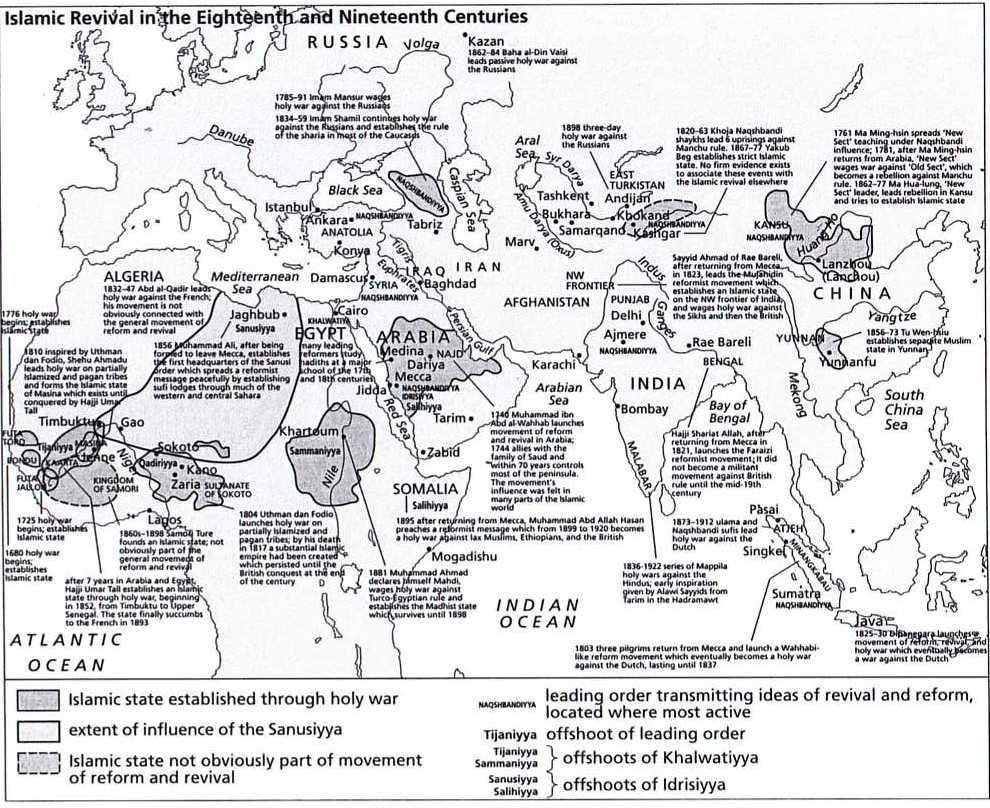
\includegraphics[width=6.59859in,height=5.38667in]{Image/media/image1.jpeg}

\begin{quote}
\emph{L'atlas de l'islam depuis 1500}, F. Robinson, Nathan, 1987
\end{quote}

\hypertarget{soufis-du-badakhshuxe2n-un-renouveau-confruxe9rique-entre-linde-et-lasie-centrale}{%
\subsection{« Soufis du Badakhshân : un renouveau confrérique entre
l'Inde et l'Asie centrale
»}\label{soufis-du-badakhshuxe2n-un-renouveau-confruxe9rique-entre-linde-et-lasie-centrale}}

\begin{quote}
Alexandre Papas, \emph{Cahiers d'Asie Centrale}, n° 11-12, 2004, p.
87-102 (extraits -- texte expurgé)
\end{quote}

\hypertarget{uxe9luxe9ments-de-biographie-dun-soufi-badakhshuxe2nais}{%
\subsection{Éléments de biographie d'un soufi
badakhshânais}\label{uxe9luxe9ments-de-biographie-dun-soufi-badakhshuxe2nais}}

\begin{quote}
Mawlânâ Mîr Ghiyâs al-Dîn naît en 1117/1705-06 dans la petite localité
de Hisârak, située au cœur du district de la ville de Jirm. Le
grand-père de Mawlânâ a émigré du village de Dahbîd, non loin de
Samarcande, en direction du Badakhshân. La \emph{silsila} de la famille
remonte au Prophète et, sur dix générations, au frère d'un grand saint
Kubrawî et découvre une généalogie soufie. C'est donc au sein d'une des
grandes familles \emph{muhâjir} de l'aristocratie religieuse du
Badakhshân que naît Ghiyâsî.

{[}\ldots{]}

C'est précisément pour l'Inde -- destination qui concurrence la
Transoxiane savante, en particulier Boukhara, surtout depuis le XVIe
siècle -- que part le jeune Ghiyâsî âgé de 14 ans en quête d'initiation.
Cet exil de l'adolescent fait l'objet de deux contes hagiographiques :
\end{quote}

\begin{itemize}
\item
  \begin{quote}
  Le futur shaykh de Ghiyâsî, Shâh Walî Allâh, qui a quitté Sirhind pour
  entreprendre un pèlerinage au mausolée de Bahâ' al-Dîn Naqshband non
  loin de Boukhara, stationne au Badakhshân, à Jirm, chez le père même
  de Ghiyâsî. Le shaykh demande alors à ce dernier de lui amener ses
  enfants, mais perçoit par claire-vue qu'on lui dissimule le jeune
  Mawlânâ qui, en état de majzûb « ravi en Dieu », suscite la honte de
  sa famille. À sa vue le shaykh indien cite un vers de Ni'mat Allâh
  Walî Kirmânî. Et au jeune Ghiyâsî de prononcer miraculeusement le
  second vers du distique. Walî Allâh annonce alors qu'à son retour de
  Boukhara il prendra le jeune homme comme disciple et l'emmènera en
  Inde.
  \end{quote}
\item
  \begin{quote}
  Dès l'âge de 9 ans Mawlânâ refuse les conseils de sa famille et se
  distingue des autres enfants. Plusieurs nuits, au cours de rêves, lui
  apparaît un homme illuminé qui lui enjoint de partir pour l'Inde où
  lui est promise la rencontre d'un grand saint soufi. Malgré le refus
  de ses parents qui souhaitent marier leur fils, Ghiyâsî parvient à
  quitter le Badakhshân quelques années plus tard. Parvenu à Lahore et
  après un nouveau rêve révélateur, il attend de nombreux jours au
  couvent de Khwâja Khwândamîr, un khalîfa de la Naqshbandiyya, jusqu'au
  jour où il rencontre Shâh Walî Allâh.
  \end{quote}
\end{itemize}

\begin{quote}
Restent les faits : après une formation classique en \emph{madrasa} à
Delhi où le novice rencontre ses premiers maîtres, il devient à Lahore
durant douze années le disciple d'un fameux maître Naqshbandî Mujaddidî.
Il interrompt une unique fois son initiation lorsque le shaykh lui
confie la mission de se rendre au Cachemire afin d'aller chercher un
homme qu'on prétend thaumaturge et que Walî Allâh souhaite convertir à
l'islam et initier à sa \emph{tarîqat}. Au terme de ses douze années de
noviciat, le shaykh lui enjoint de retourner à sa terre natale pour
propager la confrérie. De retour au Badakhshân, Ghiyâsî âgé de trente
ans environ et qui a obtenu le rang de \emph{mawlawiyyat}, fait office
d'enseignant à la \emph{madrasa} Jâmi'-i Islâmî du district de Jirm. Il
est ensuite convié à Fayz Âbâd à la cour de Sultân Shâh, laquelle abrite
des savants et des poètes venus d'Inde et d'Iran, dont certains
acquièrent grande réputation. C'est là que Ghiyâsî compose son œuvre
poétique et mystique. C'est également là, de son \emph{khânaqâh}, qu'il
dirige son enseignement, suivis par de nombreux disciples venus de
toutes les régions alentours. Le soufi badakhshânais devient aussi le
directeur spirituel de Sultân Shâh. Et lorsque ce dernier est capturé à
Qunduz par les ouzbeks du Qataghân en 1179/1765, le vieux maître
conseille durant trois ans le fils et suppléant du shah emprisonné, Mîr
Muhammad Shâh. D'un tel succès et d'une telle influence, Ghiyâsî
apparaît comme l'un des principaux promoteurs de la Mujaddidiyya dans le
Nord de l'Afghanistan.

{[}\ldots{]}
\end{quote}

\hypertarget{savants-et-soufis-au-croisement-du-badakhshuxe2n}{%
\subsection{Savants et soufis au croisement du
Badakhshân}\label{savants-et-soufis-au-croisement-du-badakhshuxe2n}}

\begin{quote}
Malgré les obstacles géographiques et en dépit des troubles politiques
qui affectent la fin du XVIII\textsuperscript{e} siècle, le Badakhshân
reçoit la visite de savants religieux qui, pour certains, décident de
s'y installer et interrompent définitivement leur voyage vers l'Inde ou
vers la Transoxiane. Il faut rappeler ici que le Pamir a, de façon
continue dans l'histoire, servi de sanctuaire à des individus frappés
d'ostracisme

ou fuyant la répression dans leur région natale. Mais au cours du
XVIII\textsuperscript{e} siècle le sanctuaire se mue en lieu de
renaissance où fleurissent \emph{madrasa} et couvent soufis. Le
\emph{Armaghân-i Badakhshân} mentionne le cas de deux étudiants de
Peshawar, Mîr Ahmad Mujaddidî dit `Izhâr' (m. 1259/1843) et son frère
Muhammad Anwar qui, à une date indéterminée durant le règne de Mîr
Muhammad Shâh, se rendent d'abord à Boukhara afin d'obtenir les
compétences du rang de \emph{`âlim} et qui, lors de leur retour,
s'installent et officient au Badakhshân, pour le premier à Jirm, pour le
second à Bahârak.

Un autre cas de figure est celui, analogue à Ghiyâsî, de ces
badakhshânais qui partent se former aux sciences religieuses, et
éventuellement au soufisme, dans les grands centres de savoir du monde
musulman, proches ou lointains. De ce point de vue, le cas le plus
intéressant -- et malheureusement le plus douloureux faute
d'informations suffisantes et dans l'absence de vestiges de son œuvre --
est celui de Sayyid Abâ al-Hasan « `Unwân ». Né à Jirm en 1123/1711, il
quitte le Badakhshân pour Boukhara afin d'acquérir une formation
théologique. De là `Unwân se rend au pèlerinage de La Mecque et à
Médine, puis il s'installe durant 18 ans en Egypte, probablement au
Caire, où il poursuit son acquisition des sciences islamiques classiques
et commence à enseigner. Mais `Unwân ne se contente pas de dispenser un
enseignement religieux, il prend parti pour les classes populaires
égyptiennes et contre leur oppression par les propriétaires terriens.
C'est du moins la réputation qu'il gagne selon le \emph{Armaghân-i
Badakhshân}, et qui lui vaut d'être banni d'Egypte. `Unwân part alors
pour Istanbul, rejoint Boukhara et reprend son enseignement. `Unwân, qui
prône l'unité de la Communauté des Croyants (\emph{umma}), décide
d'aller prêcher la concorde (\emph{âshtî}) dans le Caucase, peut-être au
moment de l'activisme Naqshbandî de Shaykh Mansûr dans les années 1780.
Mais il renonce à son projet et entre dans une retraite spirituelle
jusqu'à sa mort en 1206/1791, sans être retourné au Badakhshân.
{[}\ldots{]}

Les courants de l'islam contemporain (3)
\end{quote}

\begin{enumerate}
\def\labelenumi{\Roman{enumi}.}
\item ~
  \hypertarget{muhammad-ibn-al-wahhab-1702-1792}{%
  \subsection{Muhammad Ibn al Wahhab
  (1702-1792)}\label{muhammad-ibn-al-wahhab-1702-1792}}

  \begin{enumerate}
  \def\labelenumii{\arabic{enumii}.}
  \item
    \begin{quote}
    Formation et premières prédications
    \end{quote}
  \item
    \begin{quote}
    L'alliance avec Ibn Se`ud
    \end{quote}
  \end{enumerate}
\item ~
  \hypertarget{la-doctrine-wahhabite}{%
  \subsection{La doctrine wahhabite}\label{la-doctrine-wahhabite}}
\end{enumerate}

\begin{enumerate}
\def\labelenumi{\arabic{enumi}.}
\setcounter{enumi}{4}
\item
  \begin{quote}
  Nécessité du retour aux sources
  \end{quote}
\item
  \begin{quote}
  Une notion centrale : le \emph{tawhid} (unicité divine)
  \end{quote}
\item
  \begin{quote}
  La question du \emph{jihad}
  \end{quote}
\end{enumerate}

\begin{enumerate}
\def\labelenumi{\Roman{enumi}.}
\setcounter{enumi}{2}
\item ~
  \hypertarget{le-devenir-du-wahhabisme}{%
  \subsection{Le devenir du wahhabisme}\label{le-devenir-du-wahhabisme}}

  \begin{enumerate}
  \def\labelenumii{\arabic{enumii}.}
  \item
    \begin{quote}
    Le wahhabisme et l'Etat saoudien
    \end{quote}
  \item
    \begin{quote}
    Une étude de cas : le wahhabisme en Afrique de l'Ouest
    \end{quote}
  \end{enumerate}
\end{enumerate}

\hypertarget{glossaire-1}{%
\subsection{\texorpdfstring{\underline{Glossaire}}{Glossaire}}\label{glossaire-1}}

\begin{quote}
\underline{Personnes} `Abd al --`Aziz Abu Bakr

al-Majmu`i al-Sindi

Ibn Taymiyya Muhammad Ibn Se`ud

\underline{Lieux}

al-Azhar al-Dir'iyah

al-Uyaynah (Najd). Basra

Hijaz Huraymila Jeddah Najd

\underline{Notions}

ashraf : \emph{descendants du Prophète}

da`wa \emph{: prédication}

fiqh : \emph{droit musulman}

hadith \emph{: fait ou dire du Prophète}

hijra : \emph{« exode »}

ijma\emph{` : consensus des ulamas}

ijtihad : \emph{effort d'interprétation}

kufr \emph{: incroyance /} kafir \emph{: infidèle, mécréant}

qiyas \emph{: raisonnement par analogie}

salat : \emph{prière rituelle} shirk : \emph{associationnisme} taqlid
\emph{: imitation (servile)} tawhid : \emph{unicité divine} zakat :
\emph{aumône légale}
\end{quote}

\hypertarget{les-trois-etats-saoudiens}{%
\section{Les trois Etats Saoudiens}\label{les-trois-etats-saoudiens}}

\begin{itemize}
\item
  \begin{quote}
  \textbf{\underline{1744 -1818}: une première expansion}
  \end{quote}
\end{itemize}

\begin{longtable}[]{@{}
  >{\raggedright\arraybackslash}p{(\columnwidth - 2\tabcolsep) * \real{0.15}}
  >{\raggedright\arraybackslash}p{(\columnwidth - 2\tabcolsep) * \real{0.85}}@{}}
\toprule
\begin{minipage}[b]{\linewidth}\raggedright
\begin{quote}
\emph{1744}
\end{quote}
\end{minipage} & \begin{minipage}[b]{\linewidth}\raggedright
\begin{quote}
alliance Ibn Se`ud /Ibn al-Wahhab
\end{quote}
\end{minipage} \\
\midrule
\endhead
\begin{minipage}[t]{\linewidth}\raggedright
\begin{quote}
\emph{1786}
\end{quote}
\end{minipage} & \begin{minipage}[t]{\linewidth}\raggedright
\begin{quote}
conquête du Najd (`Abd-al-`Aziz)
\end{quote}
\end{minipage} \\
\begin{minipage}[t]{\linewidth}\raggedright
\begin{quote}
\emph{1792}
\end{quote}
\end{minipage} & \begin{minipage}[t]{\linewidth}\raggedright
\begin{quote}
mort d'Ibn al-Wahhab
\end{quote}
\end{minipage} \\
\begin{minipage}[t]{\linewidth}\raggedright
\begin{quote}
\emph{1806}
\end{quote}
\end{minipage} & \begin{minipage}[t]{\linewidth}\raggedright
\begin{quote}
conquête de La Mecque
\end{quote}
\end{minipage} \\
\begin{minipage}[t]{\linewidth}\raggedright
\begin{quote}
\emph{1818}
\end{quote}
\end{minipage} & \begin{minipage}[t]{\linewidth}\raggedright
\begin{quote}
défaite devant les Ottomans
\end{quote}
\end{minipage} \\
\bottomrule
\end{longtable}

\begin{itemize}
\item
  \begin{quote}
  \textbf{\underline{1821-1883}: petit Etat centré sur Riyad (Najd)}
  \end{quote}
\item
  \begin{quote}
  \textbf{\underline{1901- 2011} : le Royaume d'Arabie Saoudite}
  \end{quote}
\end{itemize}

\begin{quote}
\emph{1924} conquête de La Mecque. Abdelaziz Ibn Se`ud prend le titre de
roi.

\emph{1939} début de la production pétrolière \emph{1962} création de la
Ligue islamique \emph{1990} début de la guerre du Golfe.
\end{quote}

\hypertarget{larabie-saoudite-et-luxe9conomie-puxe9troliuxe8re}{%
\section{L'Arabie Saoudite et l'économie
pétrolière}\label{larabie-saoudite-et-luxe9conomie-puxe9troliuxe8re}}

\hypertarget{duxe9but-de-la-production}{%
\subsection{\texorpdfstring{\underline{Début de la
production}}{Début de la production}}\label{duxe9but-de-la-production}}

\begin{quote}
1935: premier forage

1939: premier baril de pétrole

⇒ Cartel américain: l'ARAMCO
\end{quote}

\hypertarget{nationalisation-de-la-production}{%
\subsection{\texorpdfstring{\underline{Nationalisation de la
production}}{Nationalisation de la production}}\label{nationalisation-de-la-production}}

\begin{quote}
1973: l'Etat s'approprie 25 \% des droits de l'ARAMCO
\end{quote}

\begin{longtable}[]{@{}
  >{\raggedright\arraybackslash}p{(\columnwidth - 14\tabcolsep) * \real{0.19}}
  >{\raggedright\arraybackslash}p{(\columnwidth - 14\tabcolsep) * \real{0.09}}
  >{\raggedright\arraybackslash}p{(\columnwidth - 14\tabcolsep) * \real{0.12}}
  >{\raggedright\arraybackslash}p{(\columnwidth - 14\tabcolsep) * \real{0.26}}
  >{\raggedright\arraybackslash}p{(\columnwidth - 14\tabcolsep) * \real{0.09}}
  >{\raggedright\arraybackslash}p{(\columnwidth - 14\tabcolsep) * \real{0.09}}
  >{\raggedright\arraybackslash}p{(\columnwidth - 14\tabcolsep) * \real{0.09}}
  >{\raggedright\arraybackslash}p{(\columnwidth - 14\tabcolsep) * \real{0.07}}@{}}
\toprule
\begin{minipage}[b]{\linewidth}\raggedright
\begin{quote}
1974: «
\end{quote}
\end{minipage} & \begin{minipage}[b]{\linewidth}\raggedright
«
\end{minipage} & \begin{minipage}[b]{\linewidth}\raggedright
\begin{quote}
«
\end{quote}
\end{minipage} & \begin{minipage}[b]{\linewidth}\raggedright
60 \% «
\end{minipage} & \begin{minipage}[b]{\linewidth}\raggedright
«
\end{minipage} & \begin{minipage}[b]{\linewidth}\raggedright
«
\end{minipage} & \begin{minipage}[b]{\linewidth}\raggedright
«
\end{minipage} & \begin{minipage}[b]{\linewidth}\raggedright
«
\end{minipage} \\
\midrule
\endhead
\begin{minipage}[t]{\linewidth}\raggedright
\begin{quote}
1980: «
\end{quote}
\end{minipage} & « & \begin{minipage}[t]{\linewidth}\raggedright
\begin{quote}
«
\end{quote}
\end{minipage} & 100\% « & « & « & « & « \\
\bottomrule
\end{longtable}

⇒ Saoudi ARAMCO: 95 \% de la production du pays.

\hypertarget{evolution-du-cours-du-puxe9trole}{%
\subsection{\texorpdfstring{\underline{Evolution du cours du
pétrole}}{Evolution du cours du pétrole}}\label{evolution-du-cours-du-puxe9trole}}

\begin{quote}
1973: premier choc pétrolier (guerre de Kippour) =\textgreater{} de 4 à
15 \$/B

1981-1983: deuxième choc pétrolier (Révolution iranienne + guerre
Iran-Irak) =\textgreater{} 36 \$/B 2006-2008: troisième choc pétrolier
(guerre en Irak) =\textgreater142 \$/baril
\end{quote}

\textbf{\underline{Rente}}: 1973-2002 =\textgreater{} 200 000 milliards
de dollars au total

\hypertarget{extraits-du-kitab-at-tawid-livre-de-lunicituxe9-divine-de-muhammad-ibn-wahhab}{%
\subsection{\texorpdfstring{Extraits du \emph{Kitab at-tawid} (Livre de
l'unicité divine) de Muhammad Ibn
Wahhab}{Extraits du Kitab at-tawid (Livre de l'unicité divine) de Muhammad Ibn Wahhab}}\label{extraits-du-kitab-at-tawid-livre-de-lunicituxe9-divine-de-muhammad-ibn-wahhab}}

\begin{quote}
(Traduction et édition établies en Arabie Saoudite)

\textbf{\underline{Chapitre 1} : \emph{Tawhid}}

\emph{Allah-ta`ala} a dit : « Je n'ai créé les djinns et les hommes que
pour qu'ils M'adorent (1 :56)\ldots Et très certainement nous avons
suscité dans chaque communauté un message pour leur dire d'adorer Dieu
et d'écarter le Rebelle (16 :36)\ldots Et voilà que ton Seigneur a
décrété que tu dois n'adorer que Lui et faire preuve de bonté envers tes
parents (17 :23)\ldots Adorez Dieu et ne lui donnez quelque associé que
ce soit (4 :36)\ldots Venez, je vais vous réciter ce que votre Seigneur
vous a interdit ; - ceci : Ne lui associez quoi que ce soit\ldots(6
:151-153) ». Ibn Mas`ud a dit : « Quiconque se propose de vérifier le
testament du Prophète Muhammad (SWA) -- un testament sur lequel le
Prophète a apposé son sceau, qu'il lise ces mots d'Allah : « Venez, je
vais vous réciter ce que votre Seigneur vous a interdit ; - ceci : Ne
lui associez quoi que ce soit\ldots Voilà ce qu'il enjoint » (6 :
151-153)

Mu`adh Ibn Jabal raconta : « Je montai derrière le Prophète (SAW) quand
il me dit : « Ô Mu`adh ! Sais-tu ce que les créatures d'Allah Lui
doivent et ce qui leur est dû ? » Je répondis : « Allah et son Prophète
savent mieux ». Il continua : « Ce que les créatures d'Allah Lui
doivent, c'est de ne jamais associer qui que ce soit avec Lui. Ce qui
leur est dû, c'est qu'il ne punira aucune personne qui ne Lui associe
pas un autre ». Je dis :

« Ô Prophète d'Allah, est-ce que je peux annoncer la bonne nouvelle aux
gens ? » Il répliqua : « Non ! Ne leur dis rien de peur qu'ils comptent
sur la promesse et manquent à leurs devoirs envers Lui ». Ce hadith est
mentionné dans deux \emph{Sahihs}.

D'autres points :
\end{quote}

\begin{enumerate}
\def\labelenumi{\arabic{enumi}.}
\item
  \begin{quote}
  La sagesse dans la création du djinn et de l'humanité.
  \end{quote}
\item
  \begin{quote}
  Le service à Allah consiste en le \emph{tawhid}. Car, à l'opposé du
  \emph{tawhid} se trouve l'aliénation d'Allah. (\ldots)
  \end{quote}
\item
  \begin{quote}
  La sagesse d'envoyer des prophètes. (\ldots)
  \end{quote}
\end{enumerate}

\begin{quote}
\textbf{\underline{Chapitre 2} : Les vertus du \emph{tawhid} et les
nombreux péchés qu'il expie}

\emph{Allah-ta`ala} dit : « Ceux qui ont cru et n'ont point revêtu de
prévarication leur foi\ldots{} » (6 : 82).

(\ldots) Abu Sa`id al Khudriyy rapporta que le Prophète d'Allah (SWA) a
dit : « Quand Musa {[}Moïse{]} demanda à Allah de lui enseigner une
prière qu'il puisse réciter à chaque fois qu'il pensait à Lui ou qu'il
L'évoquait, Allah répondit : « Dis, ô Musa, qu'il n'y a d'autre Dieu
qu'Allah. Musa dit : « Ô Seigneur, tous tes serviteurs prononcent ces
mots ». Allah dit : « Ô Musa, si les sept cieux et tout ce qu'ils
renferment, et les sept terres aussi, si tout cela était pesé contre
cette phrase : « Il n'y a d'autre Dieu qu'Allah », cette dernière
pèserait plus lourd ». Ibn Hibban rapporta cela également et al-Hakim
compléta sa version. Al-Tirmidhi enregistra, avec peu de rédaction, le
récit de Anas à l'effet qu'il entendit le Prophète d'Allah (SWA) dire :
« Allah dit : « Ô Homme ! Si tu venais à Moi avec tous les sacs du monde
remplis de tes péchés, mais avec le témoignage que tu n'associes rien à
Moi, Je viendrais à toi avec tous mes sacs remplis de miséricorde et de
pardon ! ».

\textbf{\underline{Chapitre 4} : La crainte du \emph{shirk}}

Allah -- qu'Il soit loué et glorifié -- dit : « Non, Dieu ne pardonne
pas qu'on Lui donne quelque associé. En deçà, Il pardonne à qui il veut
» (4 : 48, 116)

(\ldots) Dans le hadith, nous lisons : « Ce que je crains le plus pour
vous, c'est le moindre \emph{shirk}. Quand on lui demanda ce que
c'était, le Prophète répondit : « l'hypocrisie ». Dans le Sahih
d'al-Bukhari, nous lisons que Ibn Mas`ud reporta : « Le Prophète d'Allah
(SWA) a dit : « Celui qui rencontre Allah le jour du Jugement sans Lui
avoir associé qui que ce soit ira au Paradis, et celui qui le rencontre
ayant fait le contraire sera consigné en Enfer ».

\textbf{\underline{Chapitre 5} : L'appel à témoigner qu'il n'y a d'autre
Dieu qu'Allah}

\emph{Allah-ta`ala} a dit : « Dis (ô Muhammad) : `\,`Voici mon sentier,
j'appelle à Dieu'\,' » (12 :108)

Ibn `Abbas (RA) rapporta : « Quand le Prophète d'Allah (SAW) envoya
Mu'adh à al-Yaman, il lui recommanda : `\,`Quand tu rencontres des gens
du Livre, que ta première action soit de leur demander de témoigner
qu'il n'y a d'autre Dieu qu'Allah'\,' ». Selon un autre récit, «
\ldots{} de leur demander de réaliser l'unicité d'Allah. S'ils
t'obéissent, informe-les qu'Allah leur a imposé la \emph{salat} cinq
fois par jour. S'ils t'obéissent en cela, alors informe-les qu'Allah
leur a imposé le devoir de charité qui doit être perçue des riches pour
être distribué aux pauvres. S'ils t'obéissent en cela, ne touche pas à
leurs autres biens et occupe-toi de la plainte de

l'opprimé, car il n'y a aucun obstacle dans son accès à Allah ».
(Rapporté dans les \emph{Sahihs} d'al-Bukhari et de Muslim). (\ldots)

\textbf{\underline{Chapitre 17} : L'intercession}

Allah -- qu'il soit loué et glorifié -- a dit : « Et par ceci (le
Qur'an), avertis ceux qui, n'ayant pour eux hors de Dieu, ni ami ni
intercesseur, craignent d'être rassemblés vers le Seigneur\ldots{} » (6
: 51). Dis : « A Dieu l'intercession tout entière\ldots{} » (39 : 44).
Qui peut intercéder auprès de Lui que par sa permission ?... (2 : 255).
Et combien d'anges dans les cieux ? Leur intercession ne met au large en
rien, sauf après que Dieu l'a permis, en faveur de qui il veut et qu'il
agrée » (53 : 26). (\ldots)

(\ldots) En tant que catégorie générale du Jour du Jugement en laquelle
les mécréants croient, l'intercession est rejetée par le Qur'an. Le
Prophète (SAW) nous informa qu'en ce jour « il sera amené devant Allah.
Il se prosternera lui-même et louera Allah, plutôt que de demander à
intercéder. Alors on lui dira : « Lève-toi ! Parle maintenant et tu
seras entendu ! Demande et il te sera donné ! Intercède et il te sera
accordé ! » (\ldots) L'intercession est donc là pour les croyants
sincères et candides. Elle n'est accordée que par la permission d'Allah
et n'appartient pas aux associationistes. (\ldots)

\textbf{\underline{Chapitre 20} : Condamnation de celui qui invoque Dieu
auprès de la tombe du juste et, a fortiori, de celui qui invoque ce
dernier.}

Dans le \emph{Sahih}, A'ishah (RAA) rapporta : « Umm Salmah raconta au
Prophète d'Allah (SAW) qu'elle avait vue une église remplie d'images et
de statues en Abyssinie. Le Prophète dit : « Ceux-là sont les pires de
tous les hommes : lorsqu'un membre juste et vertueux de leur groupe
meurt, ils bâtissent une église sur sa tombe et y installent toutes
sortes d'images pour lui. Ils sont coupables de deux méfaits : celui
d'invoquer quelqu'un auprès d'une tombe et celui d'installer des images
». (\ldots)

Ainsi le Prophète interdit cette pratique et condamna celui qui la
suivait. Faire le \emph{salat} sur une tombe est également interdit,
même si aucune mosquée n'a été construite sur l'emplacement. Telle est
la signification de la déclaration suivante : « On craignait qu'elle ne
soit prise pour une mosquée ». Les Compagnons n'étaient pas supposés
construire une mosquée autour de la tombe du Prophète. Tout endroit
destiné au \emph{salat} ou tout endroit où le \emph{salat} est accompli,
est une mosquée. Tel l'a déclaré le Prophète (SAW) : « Toute la terre
est pour moi une mosquée, un endroit pur (pour accomplir le
\emph{salat}) ».

\textbf{\underline{Chapitre 27} : Les motivations mondaines sont des
exemples de \emph{shirk}}

\emph{Allah ta'ala} a dit : « Qui aspire à la vie d'ici-bas et à ses
parures, nous leur solderons ce qu'ils y auront fait : ils ne subiront
pas de perte ! Voilà ceux qui, dans la vie dernière, n'ont pour partage
que le Feu : leurs réalisations d'ici-bas ont crevé ! Nulles sont leurs
œuvres ! (11 : 15-16).

Abu Hurayrah (RAA) rapporta ce hadith \emph{sahih} suivant : « Le
prophète d'Allah (SAW) a dit : `\,`Malheur à l'esclave du dinar !
Malheur à l'esclave du dirham ! Malheur à l'esclave du khamilah !
(\ldots)

\textbf{\underline{Chapitre 38} : Obéir aux ulamas ou aux gouvernants
qui légitiment ce qui est interdit ou interdisent ce qui est légitime,
c'est les associer à Allah.}

Ibn `Abbas a dit : « Je vous dis que `\,`le Prophète d'Allah (SAW) a dit
ceci et vous dites que `Abu Bakr et `Umar ont dit quelque chose d'autre
?'\,' Le ciel va bientôt vous cracher des pierres sur la tête !! »

Ahmad ibn Hanbal a dit : « Très étranges, en effet, sont ceux qui,
sachant le véritable \emph{isnad} (d'un commandement du Prophète), se
tiennent quand même à l'opinion de Sufyan. Allah lui-même a dit : « Que
ceux donc qui s'opposent à son commandement prennent garde qu'une
tentation ne les atteigne, ou que ne les atteigne un châtiment
douloureux ». (24 : 63). Savez-vous ce que peut être une telle tentation
? C'est le \emph{shirk}. Car, désobéir au Prophète dans certains de ses
commandements, c'est pratiquement comme si on reniait son message et on
s'attirait le Feu.

Les courants de l'islam contemporain (4)
\end{quote}

\begin{enumerate}
\def\labelenumi{\Roman{enumi}.}
\item
  \begin{quote}
  \textbf{Les « Occidentalisants »}
  \end{quote}
\item
  \begin{quote}
  \textbf{Trois grands réformistes}
  \end{quote}
\item
  \begin{quote}
  \textbf{Foi et raison}
  \end{quote}
\item
  \begin{quote}
  \textbf{Retour aux sources et \emph{ijtihad}}
  \end{quote}
\item ~
  \hypertarget{laction-politique-et-uxe9ducation}{%
  \section{L'action: politique et
  éducation}\label{laction-politique-et-uxe9ducation}}
\end{enumerate}

\hypertarget{glossaire-2}{%
\subsection{\texorpdfstring{\underline{Glossaire}}{Glossaire}}\label{glossaire-2}}

\begin{quote}
\underline{Personnes}

Ibn Taymiyya

Jamal ad-din Al-Afghani (1839-1897) Khayr-ad din Pacha (1820- 1889)

Muhammad `Abduh (1849-1905) Seyyed Ahmad Khan (1817-1898) Shah Walli
Allah

Tahtawi (1801-1873)

\underline{Lieux}

Al-Azhar Aligarh

\underline{Autres noms propres} naqshbandi

al-`Urwa al-Wuthqa mu`tazilite nayshariyya

\underline{Notions}

bid\emph{`}a \emph{: innovation}

fiqh \emph{: droit musulman}

hadith \emph{: fait ou dire du Prophète}

\emph{`}ibadat \emph{: culte ( et partie du droit traitant du culte)}

ijma\emph{` : consensus des ulamas}

ijtihad \emph{: effort d'interprétation}

maslaha \emph{: intérêt général, bien commun}

mu\emph{`}amalat \emph{: relation (et partie du droit traitant des
relations humaines)} mufti \emph{: religieux chargé d'interpréter et de
faire appliquer la Loi musulmane} qasd \emph{: intention}

shura \emph{: principe de consultation} talfiq \emph{: interprétation
éclectique} taqlid \emph{: imitation (servile)}
\end{quote}

\hypertarget{muhammad-abduh-1849-1905}{%
\subsection{\texorpdfstring{\underline{Muhammad `Abduh}
(1849-1905)}{Muhammad `Abduh (1849-1905)}}\label{muhammad-abduh-1849-1905}}

\begin{quote}
Quand les religions firent leur apparition, les êtres humains ne
comprenaient leur intérêt, général ou particulier, que de la façon la
plus rudimentaire, plutôt comme des enfants nouveau-nés qui ne
connaissent que ce qui leur tombe sous les sens et ne distinguent
qu'avec difficulté entre le présent et le passé. Ils ne reconnaissent
vraiment que ce qu'ils touchent manuellement et leur état de conscience
ne leur permet pas de "sympathiser" avec leur famille ou leurs
compagnons, tant ils sont obnubilés par leur survie pour pouvoir
s'intéresser aux implications de leur relation aux autres, à moins qu'il
ne s'agisse d'une main qui les nourrit ou les remet sur leur pieds. Dans
ce contexte, les religions ne pouvaient s'adresser intelligemment aux
hommes en abordant les subtiles dimensions de la conscience ou en leur
faisant étalage de preuves rationnelles. Au contraire, la grande grâce
de Dieu se voit dans la manière dont ces religions s'adressèrent aux
peuples comme à des enfants, à la façon de parents qui éduquent leur
enfant avec la plus grande simplicité en se servant des sens de l'ouïe
et de la vue. Les religions prirent les hommes et leur donnèrent des
commandements directs ainsi que des prohibitions fermes exigeant la plus
complète obéissance. Bien que le sens et le but en pouvait être connu,
l'obéissance ne dépendait pas du degré de compréhension ni de
l'exactitude du savoir. Les religions fournirent aussi des miracles
étonnants et impressionnants et imposèrent des formes de culte adaptées
à la condition des hommes.

Au cours des siècles suivants, les peuples connurent grandeur et déclin,
progrès et régression. Ils se querellèrent et se réconcilièrent. Les
siècles apportèrent leur cortège de souffrances et une alternance
ininterrompue de prospérité et d'adversité qui suscitèrent une
sensibilité plus affinée, une conscience plus aiguë que l'on peut
utilement comparer à ce qui se passe dans les cœurs féminins ou à l'âge
de l'adolescence. Une religion survint alors qui parlait à ces
sentiments et, s'adressant tendrement à ces compassions, fit appel aux
doux émois du cœur. Elle donna aux humains les lois sacrées de
l'ascétisme, les éloignant complètement du monde et les tournant vers
une vie plus haute. Elle enseigna aux hommes à ne pas défendre leurs
droits si évidents qu'ils soient et ferma la porte du ciel aux riches.
D'autres traits du même genre caractéristiques de cette religion nous
sont bien connus. Elle établit des formes de culte divin qui
s'harmonisaient avec sa compréhension de l'être humain et le sens de son
message. Elle fut remarquablement efficace pour corriger les défauts et
chasser le mal des âmes qui lui étaient soumises. Mais seulement
quelques générations plus tard, les hommes se lassèrent, s'affaiblirent
et se détournèrent. Ils abandonnèrent ses exigences et ses préceptes les
trouvant au-dessus de leurs forces. Ils se mirent à penser que ces
commandements étaient naturellement impraticables. Même les cadres de
cette religion se mirent à faire concurrence aux rois dans leur autorité
et aux riches oisifs dans leur richesse. La grande masse du peuple
perdit sa noblesse au moyen de "l'interprétation" et, emporté par de
folles passions, introduisit toute sorte d'innovations.

Ainsi se passèrent les choses, tant dans l'activité que dans les
attitudes profondes. La pureté était oubliée et l'intégrité mise aux
enchères. Quant aux dogmes, ils furent infectés par le schisme et
l'hérésie. Les gardiens de la foi en abandonnèrent tous les principes à
l'exception d'un seul qu'ils croyaient - à tort - être le pilier
principal de leur foi et son fondement principal, à savoir
l'interdiction de l'examen rationnel de la foi et même des complexités
de l'univers ou de l'exploration des replis secrets de l'intelligence.
Ils promulguèrent le principe que la Raison et la Religion n'avaient
rien de commun, mais plutôt que la religion était l'ennemi juré de la
Science. Ce principe n'était pas laissé simplement au choix de chacun:
au contraire, ils l'imposèrent énergiquement comme la chose à faire par
tous et chacun. Ils imposèrent la doctrine avec une telle énergie qu'ils
déclenchèrent le plus honteux de tous les conflits de l'Histoire de
l'humanité, à savoir la guerre civile dans la maison de la religion pour
imposer des consignes religieuses. Ainsi furent détruits les fondements
eux-mêmes et brisées les liens internes à la communauté. La concorde, la
coopération et la paix disparurent: le schisme, la dispute et la
querelle régnèrent à leur place. Ainsi survécut l'humanité jusqu'à
l'avènement de l'islam.

Enfin la société humaine atteignit le point où l'homme parvient à sa
pleine stature, à l'aide d'une réflexion morale sur les vicissitudes
passées. L'Islam survint pour présenter son message à la Raison, pour
appeler à l'action l'esprit et l'intelligence, pour prendre l'émotion et
les sentiments comme partenaires afin de guider l'homme vers le bonheur
terrestre aussi bien que céleste. Il mit en lumière les causes des
discordes humaines et démontra que, devant Dieu, la religion était
unique à travers toutes les générations, qu'il n'y avait qu'un seul
projet divin visant à les réformer et à les purifier intérieurement.
L'Islam enseigna que le seul but des formes extérieures de culte était
de renouveler le recueillement intérieur nous centrant sur Dieu et que
Dieu ne regarde pas les apparences mais le cœur. Il demanda au croyant
de s'occuper du corps aussi bien que de l'âme, exigeant l'intégrité
extérieure aussi bien que l'intérieure qu'il rendit également
obligatoires. La sincérité devint le centre du culte et les rites ne
furent imposés que dans la mesure où ils conduisaient à la
sanctification de la personnalité morale. "En vérité, la prière préserve
les hommes du mal et des souillures". (Cor. 29,45) "L'Homme a été créé
instable {[}très inquiet{]}; quand le malheur le touche, il est abattu;
et quand le bonheur le touche, il est refuseur. Sauf ceux qui pratiquent
la Salat". (Cor 70,19-22) L'homme riche qui se souvient d'être
reconnaissant est élevé par l'Islam au même niveau que le pauvre qui
souffre patiemment. Peut-être même l'Islam lui porte-t-il une plus haute
estime encore. L'Islam, dans ses exhortations, s'adresse à l'homme comme
un sage et sobre conseiller s'adresserait à une personne mûre pour
l'appeler à mettre en œuvre toutes ses facultés, externes ou internes.
Il proclame sans équivoque que c'est là le moyen de plaire à Dieu et de
Lui montrer notre reconnaissance pour sa Grâce. Ce monde reçoit la
semence du monde à venir. Les hommes ne parviendront à leur fin ultime
qu'en se mettant à bien agir dans le présent.

L'Islam délivra la raison de toutes ses chaînes, il la libéra de
l'imitation aveugle qui l'avait asservie, il lui rendit son domaine dans
lequel elle tranche selon son jugement et sa sagesse ; toutefois elle
doit s'incliner devant Dieu seul et s'arrêter aux limites posées par la
religion; mais au-dedans de ces limites , il n'y a pas de barrière à son
activité et il n'y a pas de fin aux spéculations qui se déroulent sous
ses auspices.

Tiré de M. `Abduh, \emph{Risalat at-Tawhid} (\emph{Traité de l'Unité
divine}, Paris, 1925)

Les courants de l'islam contemporain (5)
\end{quote}

\begin{enumerate}
\def\labelenumi{\Roman{enumi}.}
\item ~
  \hypertarget{le-suxe9cularisme-dimportation-occidentale-le-moduxe8le-turc}{%
  \subsection{\texorpdfstring{\underline{Le sécularisme d'importation
  occidentale : le modèle
  turc}}{Le sécularisme d'importation occidentale : le modèle turc}}\label{le-suxe9cularisme-dimportation-occidentale-le-moduxe8le-turc}}

  \begin{enumerate}
  \def\labelenumii{\arabic{enumii}.}
  \item
    \begin{quote}
    Aux racines : les Jeunes Turcs
    \end{quote}
  \item
    \begin{quote}
    La République de Mustapha Kemal
    \end{quote}
  \end{enumerate}
\item ~
  \hypertarget{les-disciples-de-abduh}{%
  \subsection{\texorpdfstring{\underline{Les disciples de
  Abduh}}{Les disciples de Abduh}}\label{les-disciples-de-abduh}}

  \begin{enumerate}
  \def\labelenumii{\arabic{enumii}.}
  \item
    \begin{quote}
    Qasim Amin et le statut des femmes (1863-1908)
    \end{quote}
  \item
    \begin{quote}
    Ali Abderraziq et la laïcité (1888-1966)
    \end{quote}
  \end{enumerate}
\item ~
  \hypertarget{islam-nationalisme-et-ruxe9volution}{%
  \subsection{\texorpdfstring{\underline{Islam, nationalisme et
  révolution}}{Islam, nationalisme et révolution}}\label{islam-nationalisme-et-ruxe9volution}}

  \begin{enumerate}
  \def\labelenumii{\arabic{enumii}.}
  \item
    \begin{quote}
    Le nationalisme arabe
    \end{quote}
  \item
    \begin{quote}
    Islam et révolution : la naissance du parti ba`th
    \end{quote}
  \end{enumerate}
\end{enumerate}

\hypertarget{glossaire-3}{%
\subsection{\texorpdfstring{\underline{Glossaire}}{Glossaire}}\label{glossaire-3}}

\begin{quote}
\underline{Personnes}

`Abd ar-Rahman al-Bazzaz Abdullah Cevdet (journal \emph{Içtihad}) Edmond
Rabbath

Kawakibi Michel Aflaq

Muhammad `Abduh Qustantin Zurayq Rashid Rida

Ziya Gökalp

\underline{Lieux}

Al-Azhar

\underline{Autres noms propres} naqshbandi

sheyh ül islam

\underline{Notions}

ba'th : \emph{résurrection}

inqilâb : \emph{révolution}
\end{quote}

\hypertarget{ziya-guxf6kalp-1876-1924}{%
\subsection{\texorpdfstring{\underline{Ziya Gökalp
(1876-1924)}}{Ziya Gökalp (1876-1924)}}\label{ziya-guxf6kalp-1876-1924}}

\begin{quote}
Maintenant la mission des Turcs ne doit être que celle de découvrir le
passé pré islamique Turc qui est resté ancré dans le peuple et y greffer
la civilisation Occidentale dans sa totalité. Pour égaler les pouvoirs
européens militairement et dans les sciences et l'industrie, notre seule
voie de salut est d'adopter la civilisation Occidentale complètement!
(Ziya Gökalp, \textbf{Turkish Nationalism and Western Civilisation},
New-York, 1959, p. 276.)

Parmi les Turcs pré-islamiques, le patriotisme a atteint ses niveaux les
plus hauts. Dans l'avenir, comme dans le passé, le patriotisme doit être
le point de moralité le plus important pour les Turcs parce que la
nation et son âme sont en fin de compte la seule unité qui existe de
soi. La fidélité à la nation doit avoir la priorité sur la fidélité à la
famille ou la religion. Le Turkisme doit donner la priorité la plus
haute à la Nation et à la Patrie. Nous créerons une civilisation
véritable - une civilisation Turque qui suivra la croissance d'une
Nouvelle Vie. Classifier les Turcs, qui sont plus justes et plus beaux
que les Aryens, avec la race Mongole n'a aucune base scientifique. La
race Turque n'a pas dégénéré - comme d'autres races, par l'alcool et le
dérèglement des moeurs. Le sang turc est resté jeune et s'est durci
comme l'acier avec la splendeur du champ de bataille. L'intelligence
turque n'est pas usée; ses sentiments ne sont pas affaiblis. On promet
la conquête de l'avenir à la résolution Turque. (Ibid., pp. 302, 271 et
60.)

La civilisation occidentale est une suite de la civilisation de la
Méditerranée antique. Les fondateurs de la civilisation de la
Méditerranée étaient des peuples Turcs comme les Sumeriens, Scythes, le
Phoeniciens et les Hyksos. Il y a eu un Âge Touranien dans l'histoire
avant les âges antiques car les habitants les plus anciens de l'Asie
Occidentale étaient nos ancêtres. Ainsi nous faisons partie de la
civilisation Occidentale et avons part intégrale à cette civilisation.
(Ibid-, pp. 266- 7)

Quand une nation parvient aux étapes les plus hautes de son évolution,
elle trouve nécessaire de changer aussi sa civilisation. Quand les Turcs
étaient des membres d'une tribu nomade en Asie Centrale, ils ont
appartenu à la civilisation de l'Extrême-Orient. Quand ils ont passé à
l'étape de l'état Sultanesque, ils sont entrés dans le secteur de
civilisation Byzantine. Et aujourd'hui dans leur transition à l'état de
nation en tant qu'Etat séculier, ils sont déterminés à accepter la
civilisation Occidentale. (Ibid., pp. 270-1)

La grande erreur des autorités du Tanzimat\textbf{1} était leur
tentative de créer un amalgame mental composé d'un mélange d'Orient et
d'Occident. Ils n'ont pas réalisé que les deux, avec leurs principes
diamétralement opposés, ne pouvaient pas être réconciliés. La dichotomie
présente dans notre structure politique, le système double de tribunaux,
les deux types d'écoles, les deux systèmes de taxation, deux budgets,
les deux jeux de lois, sont tous les produits de cette erreur ... Toute
tentative de réconcilier Orient et Occident conduit à perpétuer des
conditions médiévales dans l'âge moderne et à essayer de les maintenir
en vie. De même qu'il était impossible de réconcilier des méthodes
janissaires avec un système militaire moderne, de même qu'il était
futile de synchroniser la médecine dépassée avec la médecine moderne,
ainsi est-il inutile de continuer, côte à côte, les vieilles conceptions
de la loi et les nouvelles ; les standards moderne d'éthique et les
traditionnels. Chaque civilisation a sa propre logique, ses propres
standards esthétiques, sa propre perspective du monde. Pour cette
raison, des civilisations différentes ne peuvent pas se mélanger
librement l'une avec l'autre. De nouveau, pour la même raison, quand une
société ne prend pas pour système une certaine civilisation dans sa
totalité, il ne réussit pas davantage à en prendre ses composantes. Même
s'il en prend quelques parties, il ne réussit pas à les digérer et à les
assimiler. Nos réformateurs des Tanzimat, qui ont échoué comprendre ce
point, prenaient toujours des demi-mesures dans ce qu'ils ont essayé de
faire. Avant qu'ils n'aient pris de mesures pour moderniser la
production nationale, ils ont voulu changer les habitudes de
consommation, les vêtements, l'alimentation, le bâtiment et les meubles.
D'autre part, on n'a même pas construit un noyau d'industrie digne des
standards européens parce que

\textsuperscript{1} Le mouvement des Tanzimat fut le premier essai de
réforme et de modernisation de l'empire Ottoman vers le milieu du
19\textsuperscript{ème} siècle.

les décideurs de la politique des Tanzimat ont essayé leurs réformes
sans en étudier les conditions et sans fixer des buts et des plans
précis. (Ibid., pp. 270-7).

Le but du Turkisme dans la loi est d'établir un système de loi moderne
en Turquie. La condition la plus fondamentale de notre succès à
rejoindre les rangs des nations modernes consiste à effectuer un
nettoyage complet de toutes les branches de notre structure légale pour
y effacer toute trace de théocratie et de cléricalisme. L'état qui est
libre de ces deux caractéristiques de l'état médiéval est appelé un état
moderne. En premier lieu, dans un état moderne, le droit de légiférer et
d'administrer directement appartient au peuple. Aucune fonction, aucune
tradition et aucun autre droit ne peuvent restreindre et limiter ce
droit. En second lieu, tous les membres de la nation moderne,
indépendamment de leur affiliation religieuse, sont considérés comme
égaux en tous points. Bref, toutes les dispositions existant dans nos
lois qui sont contraires à la liberté, à l'égalité et à la justice ainsi
que toutes les traces de théocratie et de cléricalisme doivent être
complètement éliminées. Le Turkisme est un mouvement séculier et ne peut
accepter que des mouvements de nature séculière. (Ibid., pp. 304-5).

C'est seulement au moyen de sa civilisation que l'Europe a été capable
de défaire les nations Musulmanes et est devenue le Maître du monde.
Pourquoi, alors, devons-nous hésiter à adopter cette même civilisation
qui s'est prouvée si capable de réussir ? Notre foi Musulmane ne nous
fait-elle pas un devoir de rechercher toutes les sortes de science et de
savoir comme notre Saint Prophète lui-même nous l'a dit, "Cherchez la
connaissance même si c'est en Chine," et "l'Étude est la propriété
perdue du croyant ; il doit la prendre partout où il la
trouve"?\textbf{2} Le Japon est considéré comme puissance européenne
mais nous sommes toujours considérés comme une nation Asiatique à cause
de notre retard à accepter véritablement la civilisation européenne.
(Ibid., pp. 266-7).

La terre où l'appel à la prière résonne en Turc et où ceux qui prient
comprennent la signification de leur religion ; la terre où le Coran est
appris en Turc et où chaque homme, grand ou petit, connaît parfaitement
le commandement de Dieu - Ô fils de la Turquie, cette terre est ta
Patrie!

Extraits traduits d'un ouvrage hostile au modernisme musulman:

Maryam Jameelah, \textbf{Islam and modernism}

(Md Yusuf Khan, Lahore, 1968), p. 101-107
\end{quote}

\hypertarget{michel-aflaq-1910-1989}{%
\subsection{\texorpdfstring{\underline{Michel `Aflaq
(1910-1989)}}{Michel `Aflaq (1910-1989)}}\label{michel-aflaq-1910-1989}}

\begin{quote}
Le Ba't arabe est apparu, dans la vie récente des Arabes, au milieu de
l'immobilisme, des reniements, de la recherche de l'intérêt personnel et
en pleine désintégration, le Ba't arabe est apparu comme un mouvement de
foi profonde qui polarise les cœurs purs et sains, qui attire les
volontés fortes et sincères, qui regroupe autour de lui les individus
emplis de l'amour de la Nation arabe, ceux qui ont foi en sa grandeur,
ceux qui ne se laissent pas aveugler par ses imperfections d'aujourd'hui
au point de ne plus voir son essence et les potentialités de son avenir,
ceux chez qui les illusions et les difficultés du présent n'ont pas
réussi à étouffer la volonté de travailler à révéler cette essence et à
réveiller ces potentialités. La croissance du Ba't arabe est une preuve
éclatante de foi, et une affirmation des valeurs spirituelles où la
religion prend sa source.

Mais cette qualité même, cette foi qui caractérise le Ba't arabe, c'est
elle qui lui fait comme une loi de se heurter à tous les mouvements qui
nient la foi ou se voilent sous une foi superficielle et contrefaite.
L'avènement du Ba't, il y a dix ans, fut une déclaration de guerre
ouverte au communisme en tant que mouvement matérialiste, négatif et
porteur de haine, et au nationalisme purement verbal qui était de mode,
qui représente la sécheresse, la stérilité et l'incapacité à créer, qui,
voyant dans la situation présente corrompue la vérité négative, perd
ainsi tout pouvoir clé maîtriser cette réalité. De même, il fallait
absolument s'opposer à la religiosité, courante alors, dans laquelle ces
mêmes défauts

\textsuperscript{2} Citations de deux hadiths souvent repris par les
apologètes de l'Islam pour montrer la compatibilité de la foi musulmane
avec la science. L'auteur les exploite d'une façon différente pour
inciter les lecteurs musulmans à s'ouvrir aux valeurs occidentales.

se manifestaient. Le Ba't arabe dès sa création a défié ces phénomènes
malsains et les a tous renvoyés à une seule cause, à savoir la perte de
confiance en soi. Ainsi le communisme n'est qu'éveil factice pour ceux
qui ont perdu tout contact avec l'esprit de leur nation, qui ont
désespéré de toute libération qui viendrait de cette nation elle-même et
se sont satisfaits d'une libération qui viendrait de l'extérieur,
factice et suspecte. Le nationalisme avait accepté le mal comme un état
normal, avait pris son parti de l'égoïsme, de la servitude et du
mensonge comme des valeurs stables de la société, parce que se rebeller
contre ces maux eût exigé de lui qu'il fît confiance en la capacité de
la nation à s'en libérer. La piété avait perdu tout lien avec l'esprit
et les élans qui furent dans le passé la source de la religion, et qui
en firent un mouvement de renaissance, de renouvellement et
d'édification. Elle régressa vers un état de léthargie, de conservatisme
et d'obscurantisme, état qui ouvrit la voie toute grande au pharisaïsme
et à l'exploitation.

Le Ba't arabe appela à une conception nouvelle de la vie nationale et de
la vie en général. La base de cette nouvelle conception est la foi dans
les valeurs spirituelles et humanistes, dans la valeur de l'esprit arabe
authentique. Elle se manifeste dans la rupture définitive d'avec les
maux de la réalité présente, dans la lutte contre ces maux sur une route
montante et difficile qui conduira la Nation arabe, lentement et
laborieusement, à retrouver son âme par le moyen de ce combat jusqu'au
sang contre sa situation présente. C'est pourquoi il n'y a plus place,
dans la conception du Ba't arabe, pour quelque sentiment religieux que
ce soit qui n'assumerait pas cette foi exemplaire. Le Ba't arabe, qui
est un mouvement spirituel et actif, ne peut se séparer de la religion
ni se heurter à elle, mais il rompt avec l'immobilisme, l'égoïsme et
l'hypocrisie.

Le Ba't arabe est un mouvement nationaliste qui se tourne vers tous les
Arabes quels que soient leur confession ou leur "rite", qui considère
comme sacrée la liberté de croyance, qui regarde les religions comme
également sacrées et respectables. Mais, à côté de cela, il voit dans
l'islam un aspect national qui joua un rôle important dans la formation
de l'histoire arabe et du nationalisme arabe. Et le Ba't estime que ce
côté national de l'islam est en relation étroite avec l'héritage
spirituel des Arabes et les caractères propres de leur génie. Le Ba't
arabe fut le premier mouvement à mettre ce lien en évidence et à lui
donner sa forme définitive. Il a ouvert par là une crise qui dure encore
et il a sauvé le nationalisme arabe de deux déviations : celle du
nationalisme abstrait qui conduit fatalement à l'artificiel et à la
misère, et celle du nationalisme religieux qui le conduirait à la
contradiction et à la ruine.

Or l'islam, en tant que religion, est égal aux autres religions dans
l'Etat arabe qui traite tous ses citoyens sur un pied d'égalité et
respecte leur liberté de croyance. L'islam en tant que mouvement
spirituel qui a été intimement mêlé à l'histoire des Arabes, qui a été
imprégné de leur génie, qui a permis l'avènement de leur grande
renaissance, cet islam a une place particulière dans l'esprit du
nationalisme arabe, dans sa culture et dans le mouvement de son éveil.
Toutefois, ce rôle n'est absolument pas imposé, mais il naît de la
liberté, de la puissance de l'esprit, de ce que les Arabes sont
extrêmement attachés et en harmonie profonde et totalement libre avec
leur esprit. C'est en ce sens que le mouvement du Ba't arabe cherche
auprès de l'islam inspiration pour son renouvellement et pour sa révolte
contre les valeurs admises dans la société. Il puise à la source de
l'islam la foi, l'idéalisme et le renoncement à l'intérêt personnel et
aux séductions de ce siècle, dans le but de répandre les principes qui
libéreront les Arabes, aujourd'hui, de leur faiblesse, de leur désunion
et de leur bas niveau spirituel et social. Enfin, le Ba't arabe tire du
dynamisme éternel de l'islam la force de résister au courant de la
réalité présente, malsaine, il y trouve un exemple admirable à suivre
pour ce qui est du zèle sincère envers l'intérêt de la Nation, quand il
s'agit de soigner ses maux avec audace, franchise, sans chercher à
flatter à peu de frais les sentiments superficiels, et sans s'appuyer
sur les forces de l'obscurantisme, de la rancœur et de l'asservissement
de l'âme et de la pensée. Le Ba't croit fermement que cette méthode, qui
est en cohérence avec les principes sublimes qu'il proclame, c'est la
méthode à laquelle le succès est assuré, comme ce fut le cas dans le
passé et comme ce le sera toujours.

Publié dans \textbf{Etudes Arabes}, N° 63, 1982-2, \emph{Courants
actuels du monde arabe, le Ba't}, p. 100-102.

Les courants de l'islam contemporain (6)
\end{quote}

\begin{enumerate}
\def\labelenumi{\Roman{enumi}.}
\item ~
  \hypertarget{au-proche-orient-arabe-uxe9mergence-des-fruxe8res-musulmans}{%
  \subsection{\texorpdfstring{\underline{Au Proche-Orient arabe} :
  \underline{émergence des Frères
  Musulmans}}{Au Proche-Orient arabe : émergence des Frères Musulmans}}\label{au-proche-orient-arabe-uxe9mergence-des-fruxe8res-musulmans}}

  \begin{enumerate}
  \def\labelenumii{\arabic{enumii}.}
  \item
    De Rashid Rida (1865-1935) à Hasan al-Banna (1906-1949)
  \item
    \begin{quote}
    Un islam « radical »
    \end{quote}
  \item
    \begin{quote}
    Un islam actif et mobilisateur
    \end{quote}
  \item
    \begin{quote}
    La question du califat et de l'Etat islamique
    \end{quote}
  \end{enumerate}
\item ~
  \hypertarget{le-thuxe9oricien-de-lislam-politique-abu-l-ala-al-mawdudi-1903-1979}{%
  \subsection{\texorpdfstring{\underline{Le théoricien de l'islam
  politique} : \underline{Abu l-a`la al-Mawdudi
  (1903-1979)}}{Le théoricien de l'islam politique : Abu l-a`la al-Mawdudi (1903-1979)}}\label{le-thuxe9oricien-de-lislam-politique-abu-l-ala-al-mawdudi-1903-1979}}

  \begin{enumerate}
  \def\labelenumii{\arabic{enumii}.}
  \item
    \begin{quote}
    Mawdudi : une vie en rupture
    \end{quote}
  \item
    \begin{quote}
    L'islam comme idéologie
    \end{quote}
  \item
    \begin{quote}
    L'islam comme utopie politique
    \end{quote}
  \item
    \begin{quote}
    L'action politique de Mawdudi
    \end{quote}
  \end{enumerate}
\end{enumerate}

\hypertarget{hasan-al-banna-1906-1949}{%
\subsection{\texorpdfstring{\underline{Hasan al-Banna
(1906-1949)}}{Hasan al-Banna (1906-1949)}}\label{hasan-al-banna-1906-1949}}

\begin{quote}
Je voudrais vous parler brièvement de la conception de l'Islam et de
l'image qu'en représentent les Frères Musulmans, pour que soit clair et
manifeste le fondement auquel nous invitons et dans lequel nous sommes
fiers de trouver notre point d'attache et notre origine.
\end{quote}

\begin{enumerate}
\def\labelenumi{\arabic{enumi}.}
\item
  \begin{quote}
  Nous, Frères Musulmans, considérons que les préceptes de l'Islam et
  ses enseignements universels intègrent tout ce qui touche l'homme en
  ce monde et dans l'autre, et que ceux qui pensent que ces
  enseignements ne touchent que l'aspect cultuel ou spirituel, à
  l'exclusion des autres, sont dans l'erreur. L'Islam est en effet foi
  et culte, patrie et citoyenneté, religion et état, spiritualité et
  action, Livre et sabre. Le noble Coran parle de tout cela, le
  considère comme substance et partie intégrante de l'Islam, il
  recommande de s'y appliquer globalement: c'est ce qu'indique ce noble
  verset: "Parmi ce que Dieu t'a donné, recherche la vie future.
  N'oublie pas ta part de ce bas-monde et sois bon comme Dieu le fut
  envers toi " (Cor. 26, 77).
  \end{quote}
\end{enumerate}

\begin{quote}
...

C'est ainsi que les Frères Musulmans ont fréquenté le Livre de Dieu,
s'en sont inspirés et guidés et sont arrivés à la conclusion que
l'Islam, c'était cette conception totale, à portée universelle et qui
devrait régir tous les aspects de la vie; ceux-ci doivent s'en
imprégner, se soumettre à son pouvoir, suivre ses préceptes et ses
enseignements, les prenant comme référence, dans la mesure où la nation
veut être authentiquement musulmane. Mais si la nation n'est musulmane
que dans son culte, suivant pour le reste d'autres modèles, cette nation
passe à côté de l'Islam. Elle ressemble à ceux que Dieu fustige:
"Croyez-vous donc à une partie du Livre et restez-vous incrédules à
l'égard d'une autre?

Quelle sera la rétribution de celui d'entre vous qui agit ainsi, sinon
d'être humilié durant la vie de ce monde et d'être refoulé vers le
châtiment le plus dur, le Jour de la Résurrection? Dieu n'est pas
inattentif à ce que vous faites" (Cor. 2, 85 b).
\end{quote}

\begin{enumerate}
\def\labelenumi{\arabic{enumi}.}
\setcounter{enumi}{1}
\item
  \begin{quote}
  De plus, les Frères Musulmans croient que la base et le soutien des
  enseignements islamiques, c'est le Livre de Dieu - qu'Il soit béni et
  exalté! - et la Tradition du Prophète - que Dieu le bénisse et lui
  donne la paix! - si une nation les prend comme règle de vie, elle ne
  saurait s'égarer. Beaucoup de théories et de sciences en contact avec
  l'Islam et qui s'en sont imprégnées portent la marque des époques qui
  les ont vues naître et des peuples qui leur furent contemporains.
  C'est pourquoi il faut puiser les lois islamiques que la nation prend
  pour référence à cette source pure, la source du premier
  jaillissement. Il importe de comprendre l'Islam comme l'ont compris
  les Compagnons et leurs successeurs de bonne souche - que la faveur de
  Dieu soit sur eux! - Il faut nous attacher à ces préceptes divins et
  prophétiques pour ne pas choisir une ligne de conduite hors de celle
  donnée par Dieu, et ne pas imposer à notre époque la marque d'une
  époque non conforme à cette ligne, l'Islam étant la religion de toute
  l'espèce humaine.
  \end{quote}
\end{enumerate}

\begin{quote}
Extraits du \emph{Message du 5ème congrès} (Le Caire, 1951) Cf.
\emph{Etudes Arabes}, n° 61, p. 35-37

***

La profession de foi des Frères musulmans (début des années 1930)
\end{quote}

\begin{enumerate}
\def\labelenumi{\arabic{enumi}.}
\item
  \begin{quote}
  Je crois que tout est sous l'ordre de Dieu ; que Muhammad est le sceau
  de toute la prophétie adressée à tous les hommes, que la Rétribution
  {[}éternelle{]} est une réalité, que le Coran est le Livre de Dieu,
  que l'Islam est une Loi complète pour diriger cette vie et l'autre. Et
  je promets de réciter {[}chaque jour{]} pour moi-même une section du
  Coran, de m'en tenir à la Tradition authentique, d'étudier la vie du
  Prophète et l'histoire des compagnons.
  \end{quote}
\item
  \begin{quote}
  Je crois que l'action droite, la vertu, la connaissance, sont parmi
  les piliers de l'Islam. Et je promets d'agir droitement en
  accomplissant les pratiques du culte et en évitant les choses
  mauvaises : je me plairai aux bonnes mœurs, j'aurai en horreur les
  mauvaises, je répandrai autant que je peux les usages musulmans, je
  préférerai l'amour et l'attachement plutôt que la rivalité et la
  condamnation, je ne recourrai aux tribunaux que contraint et forcé, je
  renforcerai les rites et la langue de l'Islam et je travaillerai à
  répandre les sciences et les connaissances utiles dans toutes les
  classes de la nation.
  \end{quote}
\item
  \begin{quote}
  Je crois que le musulman doit travailler, gagner sa vie, s'enrichir,
  et qu'une part de ses gains revient de droit au mendiant et au
  misérable, et je promets que je travaillerai pour gagner ma vie et
  assurer mon avenir, que j'acquitterai la \emph{zakât} {[}aumône{]} sur
  mes biens en en gardant aussi une part volontaire pour faire la
  charité, que j'encouragerai tout projet économique utile et ferai
  progresser les produits de ma région, de mes coreligionnaires, de ma
  patrie, sans jamais pratiquer l'usure ni l'intérêt ni chercher le
  superflu au-delà de mes capacités.
  \end{quote}
\item
  \begin{quote}
  Je crois que le musulman est responsable de sa famille, qu'il a le
  devoir de la conserver en bonne santé, dans la foi, dans les bonnes
  mœurs. Et je promets de faire mon possible en ce sens et d'insuffler
  les enseignements de l'Islam aux membres de ma famille. Je ne ferai
  pas entrer mes fils dans une école qui ne préserverait pas leurs
  croyances, leurs bonnes mœurs. Je lui supprimerai tous les journaux,
  livres, publications qui nient les enseignements de l'Islam, et
  pareillement les organisa- tions, les groupes, les clubs de cette
  sorte.
  \end{quote}
\item
  \begin{quote}
  Je crois que le musulman a le devoir de faire revivre l'Islam par la
  renaissance de ses différents peuples, par le retour de sa législation
  propre, et que la bannière de l'Islam doit couvrir le genre humain et
  que chaque musulman a pour mission d'éduquer le monde selon les
  principes de l'Islam. Et je promets de combattre pour accomplir cette
  mission tant que je vivrai et de sacrifier pour cela tout ce que je
  possède.
  \end{quote}
\item
  \begin{quote}
  Je crois que tous les musulmans ne forment qu'une seule nation unie
  parla foi islamique et que l'Islam ordonne à ses fils de faire le bien
  à tous ; je m'engage à déployer mon effort pour renforcer le lien de
  fraternité entre tous les musulmans, et pour abolir l'indifférence et
  les divergences qui existent entre leurs communautés et leurs
  confréries.
  \end{quote}
\item
  \begin{quote}
  Je crois que le secret du retard des musulmans réside dans leur
  éloignement de la religion, que la base de la réforme consistera à
  faire retour aux enseignements de l'Islam et à ses jugements, que ceci
  est possible, si les musulmans œuvrent dans ce sens, et que la
  doctrine des Frères musulmans réalise cet objectif Je m'engage à m'en
  tenir fermement à ces principes, à rester loyal envers quiconque
  travaille pour eux, et à demeurer un soldat à leur service, voire à
  mourir pour eux.
  \end{quote}
\end{enumerate}

\begin{quote}
Traduit et cité dans Olivier Carré et Gérard Michaud {[}Michel
Seurat{]}, \emph{Les Frères musulmans} (1928-1982), Paris, Archives
Gallimard/Julliard, 1983, p. 25-26.
\end{quote}

\hypertarget{abu-l-ala-al-mawdudi-1903-1979}{%
\subsection{\texorpdfstring{\underline{Abu l-a'la al-Mawdudi
(1903-1979)}}{Abu l-a'la al-Mawdudi (1903-1979)}}\label{abu-l-ala-al-mawdudi-1903-1979}}

\begin{quote}
La situation actuelle devant laquelle nous nous trouvons est, en résumé,
la suivante: les gouvernements refusent de suivre la route que la
Communauté musulmane veut suivre, et la Communauté musulmane refuse de
suivre la politique que poursuivent les gouvernements. D'où une lutte
continuelle et acharnée entre les peuples et les gouvernements, dans
tous les pays musulmans. L'Islam contemporain, c'est cela. Des efforts
colossaux sont déployés pour transformer les musulmans en non-musulmans,
et pour cela, tous les moyens possibles sont employés.

D'une façon particulière, le domaine de l'instruction et de l'éducation.
On se sert de méthodes qui sont de nature à condamner toutes les valeurs
islamiques des musulmans, à corrompre leurs mœurs et leurs goûts, à les
détourner de leur héritage culturel et de leurs traditions; elles les
encouragent à suivre une culture qui détruit ce qui reste de leur
morale, et elles répandent chez eux les disciplines occidentales,
destinées à créer en eux des doutes sur l'Islam. Le fin mot de
l'affaire, c'est que les musulmans se trouvent soudain atteints de
faiblesse, de défaillance et d'impuissance, et qu'ils deviendront un
peuple qui a perdu sa personnalité. Et cela n'est pas impossible. Mais
ce qui est impossible, c'est qu'ils renoncent délibérément à l'Islam et
qu'ils créent volontairement un Etat irréligieux.

Quant aux conséquences désastreuses de cette lutte pour les pays
musulmans, il suffit, pour en mesurer l'étendue, d'examiner la part
qu'ont prise ces pays au mouvement de la Renaissance. Voyons- nous un
seul domaine de la vie touché par le progrès? La Turquie, par exemple,
Etat indépendant doté de la souveraineté depuis 1924, jusqu'à quel point
a-t-elle réussi à développer son industrie? A quel stade est-elle
arrivée dans le domaine du commerce? alors que le Japon, qui a atteint
l'indépendance en même temps que la Turquie, est parvenu à un niveau
incroyable de développement matériel. La cause de cette situation ne
saurait échapper aux gens intelligents. La Turquie a dévié de la bonne
route et s'est tournée vers le champ clos de la lutte interne. Ses
gouvernements successifs ont essayé de faire apparaître le peuple turc
comme un peuple non-musulman; mais le peuple turc a refusé de se
transformer en un peuple non-musulman. Au contraire, il a voulu tourner
sa face vers l'Islam, ce qui a déclenché une lutte continuelle et
furieuse entre le gouvernement et le peuple. Comment la Turquie, après
cela, poursuivrait-elle sa marche en avant et s'assurerait-elle le
progrès matériel? La situation a atteint son paroxysme ces derniers
temps, quand la rupture s'est étendue à l'armée elle-même: à ce jour,
six mille officiers ont été relevés de leurs fonctions. Et ce qui est
dit de la Turquie peut être dit également des autres pays musulmans.

Soyez-en sûrs, mes frères! Partout où il y a conflit, lutte entre la
conscience du peuple et la politique du gouvernement, la stagnation y
plante ses griffes, elle empêche le peuple d'avancer, ne serait-ce que
d'un pouce, et les pas du progrès ne se dirigeront pas vers lui. Aucun
gouvernement ne peut promouvoir la force et le bien-être, sans qu'il y
ait harmonie et union entre la conscience du peuple et la politique de
ce gouvernement, de telle sorte que, quelle que soit la politique du
gouvernement, elle soit sanctionnée par les sentiments et les
aspirations du peuple. Et quand cette politique est mise on œuvre, le
peuple déploie tous ses efforts pour la faire réussir.

C'est là le seul moyen de faire du peuple un peuple actif et vigilant.
Mais dans le cas contraire, lorsque le peuple est coupé du gouvernement,
il ne bénéficie pas du moindre progrès. Il est à présumer que le peuple,
même si le gouvernement ne lutte pas pour réaliser ses aspirations, ne
se soulèvera pas contre lui; mais que le peuple s'abstienne d'assister
et de soutenir le gouvernement, cela suffit à conduire le pays vers une
catastrophe certaine. L'insatisfaction du peuple à l'égard de son
gouvernement est donc une chose grave en soi et une situation
inquiétante.

Si ces gens (du gouvernement) persistent à aller à contre-courant, c'est
uniquement par égoïsme, égocentrisme et soumission au pouvoir des
passions. Ils n'ignorent pourtant pas ce que veut le peuple. De plus,
leur expérience passée est la meilleure preuve que ce peuple ne s'est
secoué et n'a joué son rôle héroïque dans les batailles pour la
libération qu'au nom de l'Islam. Ce sursaut du peuple, qui découle de
l'Islam, a conduit les musulmans aux rivages de la liberté et à tenir
une position de force. C'est pourquoi, ces gens-là n'ignorent pas
l'attachement sûr et solide de leur peuple à l'Islam. Mais ayant lié
leur destinée et celle de leurs enfants à l'Occident, à sa civilisation
et à ses mirages, s'étant plongés dans la civilisation occidentale et
ayant mis son empreinte sur leurs coutumes et leurs goûts, ils ne
veulent pas suivre le chemin de l'Islam, et leur égoïsme les empêche
d'agir en musulmans. La logique sur laquelle ils s'appuient est la
suivante: ils ont reçu mission de gouverner leurs peuples déshérités et
malheureux, en toutes circonstances; or l'Islam, religion de ces
peuples, ne leur plaît pas; donc les peuples doivent abandonner l'Islam.
Voilà la règle universelle qu'ils ont adoptée comme fondement de leurs
activités et de leurs orientations.

Tel est l'Islam aujourd'hui. J'essaierai maintenant de définir
brièvement ce que devrait être l'Islam demain.
\end{quote}

\hypertarget{lavenir-du-monde-musulman}{%
\subsection{L'avenir du monde
musulman}\label{lavenir-du-monde-musulman}}

\begin{quote}
L'avenir du monde musulman dépendra de l'attitude que les musulmans
adopteront envers l'Islam. Si le monde de l'Islam s'en tient à son
attitude actuelle, faite d'hypocrisie, de déguisement et de duplicité,
s'il persiste dans son attitude hostile à l'Islam, je crains que les
peuples musulmans ne soient pas capables de maintenir leur indépendance
ni de la préserver de la ruine; au contraire, ils tomberont une deuxième
fois - ce qu'à Dieu ne plaise!- dans les fers de l'esclavage, et ils
iront à la rencontre d'une condition pire que celle dans laquelle ils
ont vécu précédemment, pendant la période de l'esclavage.

Oui, si ceux qui tiennent les rênes du pouvoir dans le monde musulman
retrouvent le droit chemin avant qu'il ne soit trop tard, et s'ils
travaillent à ramener la véritable vie démocratique, si le pouvoir
d'élire les dirigeants fait retour aux masses, de telle sorte qu'elles
puissent choisir qui elles veulent et confier librement les rênes du
pouvoir à ceux qu'elles aiment, et si l'ordre politique, l'économie,
l'enseignement sont en harmonie avec les principes de l'Islam, avec ses
objectifs et sa civilisation, alors je suis convaincu que les peuples
musulmans deviendront très vite une grande puissance dans le monde,
qu'ils seront capables de contrôler le pouvoir dans les instances
internationales et d'avoir le dernier mot.

L'existence du bloc des peuples musulmans ne doit pas être sous-estimée.
Ce bloc, qui s'étend de l'Indonésie à l'est jusqu'au Maroc à l'ouest,
qui est doté de moyens et de possibilités incommensurables, qui jouit
d'un capital énorme de main d'œuvre, s'il se met à suivre les principes
de l'Islam et à agir en commun en s'appuyant sur ce dernier, y aura-t-il
une force, que ce soit dans le monde occidental ou dans le monde
oriental, capable de lui résister ?

Extrait de son livre \emph{al-Islam al-yawm} (l'Islam aujourd'hui)

Trad. Roberto Bellani, parue dans \emph{Etudes Arabes}, n° 52, p. 81-83.

Les courants de l'islam contemporain (7)
\end{quote}

\begin{enumerate}
\def\labelenumi{\Roman{enumi}.}
\item ~
  \hypertarget{un-pensuxe9e-fondatrice-sayyid-qutb-1906-1966}{%
  \subsection{\texorpdfstring{\underline{Un pensée fondatrice : Sayyid
  Qutb
  (1906-1966)}}{Un pensée fondatrice : Sayyid Qutb (1906-1966)}}\label{un-pensuxe9e-fondatrice-sayyid-qutb-1906-1966}}

  \begin{enumerate}
  \def\labelenumii{\arabic{enumii}.}
  \item
    \begin{quote}
    Une vie de militant
    \end{quote}
  \item
    \begin{quote}
    Le \emph{Fi zilâl al-Qur'an} : une méthode de lecture du Coran
    \end{quote}
  \item
    \begin{quote}
    L'Etat islamique : une utopie
    \end{quote}
  \end{enumerate}
\end{enumerate}

\begin{quote}
5. Place centrale du \emph{jihad}
\end{quote}

\begin{enumerate}
\def\labelenumi{\Roman{enumi}.}
\setcounter{enumi}{1}
\item ~
  \hypertarget{les-duxe9rives-djihadistes}{%
  \subsection{\texorpdfstring{\underline{Les dérives
  djihadistes}}{Les dérives djihadistes}}\label{les-duxe9rives-djihadistes}}

  \begin{enumerate}
  \def\labelenumii{\arabic{enumii}.}
  \item
    \begin{quote}
    La première génération : la guérilla.
    \end{quote}
  \item
    \begin{quote}
    La deuxième génération : le terrorisme mondial.
    \end{quote}
  \item
    \begin{quote}
    Da`esh, troisième génération du djihadisme
    \end{quote}
  \item
    \begin{quote}
    Le martyre : quelle légitimité ?
    \end{quote}
  \end{enumerate}
\end{enumerate}

\hypertarget{glossaire-4}{%
\subsection{\texorpdfstring{\underline{Glossaire}}{Glossaire}}\label{glossaire-4}}

\begin{quote}
\underline{Personnes}

Al-Zawahiri (Ayman) Ben Laden (Usama) Farag (Abd as-salam) Ibn Taymiyya
Mawdudi

Nadawi

Qaradawi (Sheykh) Tantawi (Sheikh)

\underline{Autres noms propres} Al-Jazira/ Al-Jazeera Dar-al-ulum

Hamas

Harakat al-jihad al-islami Hezbollah

kharijites

\underline{Notions}

dar al-harb: \emph{territoire de la guerre}

dar al-islam: \emph{territoire de l'islam}

dar al-kufr: \emph{territoire des infidèles (mot-à- mot : territoire de
l'impiété)}

dar as-sulh: \emph{territoire de la paix}

dhimmi : « protégés » (statut particulier accordé aux chrétiens et aux
juifs) fasiq: \emph{pécheur}

fiqh: \emph{droit (musulman)}

fitna: \emph{discorde, querelle (conflit interne au monde musulman)}

hakimiyya : \emph{souveraineté}

hijra : \emph{exode}

`ibada : \emph{culte}

ijtihad : \emph{effort personnel d'interprétation (des textes sacrés)}

isnad : \emph{chaîne de transmission (des hadiths)} jahiliyya :
\emph{ignorance =\textgreater{} société païenne, impie}

kafir/kufr : \emph{impie/impiété}

munafiq : \emph{hypocrite (désigne l'ennemi}

\emph{« interne » à l'umma)}

na'ib : \emph{délégué} qatl : \emph{meurtre} shahid : \emph{martyr}

shura : \emph{principe de consultation}

taghut : \emph{tyran}

`ubudiyya : \emph{servitude}

umma : \emph{communauté musulmane}
\end{quote}

\hypertarget{sayyid-qutb-1906-1966}{%
\subsection{\texorpdfstring{\underline{Sayyid Qutb
(1906-1966)}}{Sayyid Qutb (1906-1966)}}\label{sayyid-qutb-1906-1966}}

\begin{quote}
UNE GENERATION CORANIQUE UNIQUE

\textbf{Il y a un phénomène historique devant lequel doivent s'arrêter
les détenteurs de l'appel de l'islam en tout lieu et en tout temps.} Et
ils doivent s'y arrêter longuement. En effet, cela a une influence
décisive sur la méthode et l'orientation de l'appel. \textbf{Cet appel a
formé une génération de gens, la génération des compagnons (que la
satisfaction de Dieu soit sur eux), une génération distinguée dans toute
l'histoire de l'Islam et dans l'histoire de l'humanité toute entière.
Depuis il n'a jamais été formé ce type {[}d'homme{]} une autre fois}.
Oui, on trouve des individus de ce type dans le cours de l'histoire,
mais il n'est jamais arrivé que se rassemble un si grand nombre, en un
seul endroit, comme il y avait dans cette première période de la
génération de cet appel. Ceci est un phénomène clair et actuel, il
possède une signification devant laquelle il faut s'arrêter longuement ;
peut-être découvrirons-nous son secret. Le Coran de cet appel est entre
nos mains ; le hadith du Messager de Dieu, (la bénédiction de Dieu et la
paix soient sur Lui), son enseignement pratique, sa noble biographie,
sont aussi entre nos mains, comme ils étaient entre les mains de cette
première génération - laquelle ne s'est pas répétée dans l'histoire-...
Rien n'a disparu {[}aujourd'hui{]}, sauf la personne du Messager de
Dieu, (la bénédiction de Dieu et la paix soient sur Lui). Alors, est-ce
cela le secret ? Si l'existence du Messager de Dieu, (la bénédiction de
Dieu et la paix soient sur Lui) était inévitable pour la mise en place
de cet appel, et pour porter ses fruits ; Dieu n'en aurait pas fait un
appel à tous les hommes, et n'en aurait pas fait un dernier message,
n'en aurait pas fait dépendre les affaires des hommes sur terre jusqu'à
la fin des temps. Mais Dieu (qu'il soit honoré) s'est engagé par la
conservation de l'invocation et il a su que cet appel pouvait continuer
après le Messager de Dieu, (la bénédiction de Dieu et la paix soient sur
Lui) et pouvait porter ses fruits. Il l'a rappelé auprès de lui après 23
ans de mission et a fait rester sa religion depuis après lui jusqu'à la
fin des temps. L'absence de la personne du Messager de Dieu, (la
bénédiction de Dieu et la paix soient sur Lui) n'explique donc pas ce
phénomène et n'en donne pas la raison.

* * *

Cherchons donc une autre cause. \textbf{Regardons la source a laquelle a
puisé cette première génération, peut-être que quelque chose a changé en
elle}. Et regardons dans la voie qui les a formés ; peut-être que
quelque chose a changé en elle pareillement.

\textbf{Cette première source a laquelle a puisé cette génération, c'est
la source du Coran. Rien que le Coran}. Alors, le hadith du Messager de
Dieu, (la bénédiction de Dieu et la paix soient sur Lui), et son
enseignement, n'ont été qu'une des traces de cette source. Et quand on a
interrogé Aïsha (que Dieu soit satisfait d'elle) au sujet de l'éthique
du Messager de Dieu, (la bénédiction de Dieu et la paix soient sur Lui),
elle a dit: ``\textbf{Son éthique était le Coran}''\textbf{Le Coran seul
donc, était la source à laquelle ils ont puisé, par laquelle ils sont
devenus conditionnés, par laquelle ils ont été formés. Ceci n'a pas été
ainsi parce qu'à ce jour, l'humanité n'avait ni civilisation, ni
culture, ni science, ni écrits, ni études... Non ! Au contraire, il y
avait la civilisation romaine, sa culture, ses lois, desquelles l'Europe
continue à vivre (ou de ses extensions)}. Et il y avait les vestiges de
la civilisation grecque, sa logique, sa philosophie, son art et c'est ce
qui continue à irriguer la pensée occidentale jusqu'à aujourd'hui. Et il
y avait de même la civilisation perse, son art, sa poésie, sa
mythologie, ses dogmes et son système de gouvernement. Et d'autres
civilisation lointaines et proches : la civilisation hindoue, la
civilisation chinoise, etc. Et les deux civilisations romaines et perses
étaient au bord de la péninsule arabique, à son nord et à son sud, de
même que les juifs et les chrétiens vivaient au coeur de la péninsule...
\textbf{Ce n'est donc pas à cause de la pauvreté des civilisations
mondiales, des cultures mondiales que cette génération s'est limitée au
Livre de Dieu uniquement, dans la période de formation. il y avait là
une intention spécifique, une direction voulue.}

La colère du Messager de Dieu, (la bénédiction de Dieu et la paix soient
sur Lui) a montré cette intention quand il a vu dans la main de Omar ben
Khatâb (que Dieu soit satisfait de lui), une copie de la Torah. Alors,
il a dit : Si Moïse avait vécu parmi vous, il ne lui aurait pas été
permis autre chose que me suivre.''\textbf{Il y avait donc l'intention
de la part du Messager de Dieu, (la bénédiction de Dieu et la paix
soient sur Lui) de limiter la source à laquelle a puisé cette
génération, dans cette première période de formation, au Livre de Dieu
uniquement, pour que leurs âmes soient pour Lui seul, et pour que leur
comportement se redresse sur sa voie à Lui seul.} D'où le fait qu'il est
devenu furieux quand il a vu Omar ben Khatâb (que Dieu soit satisfait de
lui), puiser à d'autre source. Le Messager de Dieu, (la bénédiction de
Dieu et la paix soient sur Lui) a voulu faire une génération pure de
coeur, pure d'esprit, pure d'appréhension, pure de sentiment, pure de la
formation de toute influence autre que celle de la direction divine que
contient le Saint Coran. \textbf{Cette génération a puisé donc à cette
unique source ; ce pourquoi elle a eu dans l'histoire ce statut
unique... Alors, que s'est-il passé ? Les sources se sont mélangées. Se
sont déversé dans la source à laquelle a puisé les générations
suivantes, la philosophie des grecs et leur logique, la mythologie perse
et ses conceptions, les ``judaïtés'' juive et la théologie chrétienne et
d'autres éléments d'autres civilisations et cultures. Tout cela était
mélangé avec le \emph{tafsîr} du Coran, et la science du \emph{Kalâm},
comme c'était mélangé avec le \emph{fiqh} et la croyance. Toutes les
générations, après celle-ci ont été formées à cette source polluée, si
bien que cette génération ne s'est jamais répétée}. Et il ne fait pas de
doute que le mélange de cette source première a été un des facteurs
fondamentaux de cette différence entre toutes ces générations et la
génération distincte et unique.

* * *

\textbf{Il y a un autre fait fondamental, autre que la différence de
nature de la source. C'est la manière différente de recevoir ce qui a
formé cette génération unique et distincte}. Ceux de la première
génération \textbf{ne lisaient pas le Coran avec la volonté
{[}d'acquérir{]} une culture ou un savoir, ni avec la volonté du goût et
de la jouissance. Aucun d'entre eux n'a reçu le Coran pour augmenter sa
provision de culture, juste pour la culture, et ne remplissaient une
réserve de propositions scientifiques et juridiques. En effet, il
recevait le Coran pour recevoir un ordre de Dieu concernant ses affaires
et les affaires de la communauté dans laquelle il vivait. Il recevait
cet ordre pour le mettre en pratique dès qu'il l'entendait, comme un
soldat reçoit l'ordre du jour dans un champ de bataille pour le mettre
en pratique sitôt reçu.} En conséquence, il n'y avait aucun d'entre eux
pour {[}chercher{]} à augmenter ces {[}réserves{]} d'un seul coup, parce
qu'il sentait que cela augmentait les devoirs et les fardeaux qu'il
devait charger sur ses épaules et il se limitait à dix versets afin de
les garder et d'y travailler (comme il est dit dans le hadith de Ibn
Mas'ud (que Dieu soit satisfait de lui) \textbf{Cette attitude . . .
cette attitude de recevoir pour la mise en pratique. . . leur ouvrait
dans le Coran les horizons de la joie, horizons du savoir, qui
n'auraient pas été ouverts s'ils avaient misé sur lui avec une attitude
de recherche, d'études et de connaissance. Cela rendait facile le
travail et rendait léger les fardeaux. Le Coran était mélangé avec leur
identité, était transformé dans leurs âmes et leur vie, en un chemin
concret, en une culture dynamique qui ne reste pas à l'intérieur des
esprits ni sur le papier, mais se change en effets et en événements qui
modifie la trajectoire de la vie.} Le Coran ne livre ses trésors qu'à
ceux qui viennent à lui avec cet esprit : esprit de connaissance
engendrant une pratique. Il ne vient pas pour être un livre de plaisir
intellectuel, ni un livre de lettre et d'art, ni un livre d'histoires ou
d'histoire (même si tout ceci est contenu dedans), mais il vient pour
être un chemin de vie, un chemin purement divin. Et Dieu (gloire à Lui!)
les prenait, par cette voie fragmentée, qu'ils ont suivi petit à petit.
``Et nous avons fragmenté le Coran pour que tu le récites aux gens
progressivement et nous l'avons réellement fait descendre'' (17, 106) Ce
Coran n'est pas descendu comme un tout, mais il est descendu selon les
besoins nouveaux et selon la

croissance continue des idées et des conceptions, la croissance continue
de la société et de la vie et selon les problèmes pratiques qui se
présentaient à la communauté musulmane dans sa vie concrète. Le verset
(ou les versets) descendait dans la situation particulière ou pour un
événement spécifique, parlant aux hommes de ce qui était en leur âme et
les éclairant sur ce qu'ils avaient à faire, dessinant pour eux la voie
concrète dans telle situation, corrigeant leurs fautes d'attitude et de
conduite, les rattachant en tout cela à Dieu, leur maître, Le faisant
connaître d'eux à travers ses attributs caractéristiques dans le cosmos.
Alors, ils sentaient qu'ils vivaient ici donc dans le domaine du
Très-Haut, sous l'oeil de Dieu, dans le domaine de son pouvoir. Et dès
lors, ils ont accordé les situations de leur vie selon cette authentique
voie divine. La méthode de recevoir pour la mise en pratique et l'action
est ce qui a façonné cette première génération. Et la méthode de
recevoir pour étudier et pour se réjouir est ce qui a formé les
génération qui ont suivi et il n'y a pas de doute que ce second fait est
aussi fondamental que le premier dans la différence de toutes les
générations par rapport à la génération spécifique et unique.

* * *

\textbf{Il y a un troisième fait difficile pour l'attention et la
mémorisation. L'homme qui était sur le point d'entrer dans l'Islam
abandonnait sur le seuil de la porte tout son passé de Jâhiliya}.
\textbf{Il sentait à cette seconde où il venait à l'Islam qu'il
commençait une nouvelle phase, se séparant complètement de la vie qu'il
menait dans la Jâhiliya. Et il s'arrêtait devant tout ce que comportait
sa phase de Jâhiliya ; un arrêt de suspicion, de doute, de méfiance et
de crainte; il sentait que toute cette pollution ne convenait pas pour
l'Islam !} Avec cette sensation, il recevait l'enseignement {[}de
l'Islam{]} nouveau. Et si, une fois, son inclinaison l'emportait sur lui
; si, une fois, ses {[}anciennes{]} habitudes l'attiraient; si, une
fois, il faiblissait devant les obligations musulmanes ... il sentait
immédiatement sa culpabilité et son péché et il reconnaissait du fond de
son âme qu'il avait besoin d'une purification là où il était tombé et il
essayait une nouvelle fois de vivre en accord avec l'enseignement du
Coran. Il y avait donc une attitude complète de séparation entre le
passé du musulman dans la Jâhiliya et le présent dans l'Islam. Cela
résultait d'une séparation complète de ses relations avec la société de
la Jâhiliya de ce qui l'entourait et de ses liens sociaux. Il se
séparait donc définitivement de l'environnement de la Jâhiliya, pour se
connecter finalement à l'environnement de l'Islam. Même s'il était mêlé
avec quelques polythéistes en travaillant dans le monde des affaires et
des échanges quotidiens, cette séparation d'attitude était une chose et
les échanges quotidiens une autre chose. \textbf{Il y avait un acte de
séparation de l'environnement de la Jâhiliya, de ses coutumes, de ses
conceptions, de ses habitudes, de ses liens ; qui résultait de la
séparation de la foi polythéiste pour la foi monothéiste, de la
conception de la Jâhiliya pour la conception islamique sur la vie et
l'existence.} Et cela était dû au fait d'avoir rejoint la nouvelle
assemblée islamique, ses nouveaux meneurs et d'avoir donné à cette
assemblée et à ces meneurs toute allégeance, toute obéissance et toute
communion. Et c'était ce carrefour, c'était le début d'une marche sur le
chemin nouveau, le chemin libre et allégé de toutes les pressions des
coutumes acceptées par la société de la Jâhiliya, et de toutes les
conceptions et des valeurs qui y dominent. Il n'y avait rien d'autre que
ce que le musulman rencontrait de préjudice et de mise à l'épreuve. Mais
il avait lui même tranché et y avait mis un terme, si bien que ni la
pression des conceptions de la Jâhiliya, ni les coutumes de la société
de la Jâhiliya ne pouvait l'atteindre. \textbf{Nous sommes aujourd'hui
dans la Jâhiliya, la même la Jâhiliya que celle qui était contemporaine
à l'Islam ou {[}même{]} plus sombre. Tout ce qui nous entoure est
Jâhiliya, les conceptions des gens, leurs croyances, leurs habitudes et
leurs coutumes, les sources de leur culture, leur art et leur
littérature, leurs normes et leurs lois. A tel point que beaucoup de ce
que nous considérons comme culture islamique, comme références
islamiques, comme philosophie islamique, comme pensée islamique, sont un
produit de cette Jâhiliya.} C'est pour cela que ne se dressent pas en
nos âmes les valeurs de l'Islam et que ne s'éclaire pas

en notre intelligence les conceptions de l'Islam et que la grande
génération des gens de ce type qu'a produit l'islam la première fois ne
se reproduit pas en nous. \textbf{Il nous faut donc dans cette voie du
mouvement islamique, nous dépouiller (dans cette période de gestation et
de commencement) de toutes les influences de la Jâhiliya dans lesquelles
nous vivons et desquelles nous sommes inspirés. Et nous devons retourner
à la source pure qui a inspiré ces hommes, la source garantie qui n'a
pas été mélangée et qui n'a pas été rendue impure}. Nous retournons vers
elle en y empruntant notre conception de la vérité de l'existence
entière et de la vérité de l'existence humaine et de la totalité des
relations entre ces deux existences et entre l'existence parfaite de la
vérité, existence de Dieu (loué soit-il)... Et puis, de cela nous
empruntons nos conceptions de la vie, nos valeurs morales, nos approches
pour juger de la politique, de l'économie et de tous les éléments de la
vie. Et quand on y retourne il faut y retourner avec le sentiment de
``recevoir pour mettre en pratique'' et non avec un sentiment ``d'étude
et de plaisir''. Nous y retournons pour savoir ce qu'il nous demande
d'être et pour l'être. Et sur le chemin, nous rencontrerons, la beauté
artistique dans le Coran, les belles histoires du Coran, les scènes du
jugement dernier {[}qui se trouvent{]} dans le Coran, la logique que
l'on sent dans le Coran et les autres choses que demandent les ``gens de
l'étude et du plaisir''. Mais tout cela nous le rencontrerons, sans que
cela soit notre premier but. Que notre premier but soit de connaître :
qu'est-ce que le Coran veut que nous fassions ? Quelle est la conception
globale qu'il veut que nous concevions ? Comment le Coran veut que
soient nos sentiments pour Dieu? Comment veut-il que soient nos
comportements éthiques, nos conditions, notre organisation pratique de
la vie?Alors, il nous est nécessaire de nous purifier des pressions de
la société de la Jâhiliya, des conceptions de la Jâhiliya, des coutumes
de la Jâhiliya, du commandement de la Jâhiliya, au fond de nous-même. Ce
n'est pas notre préoccupation de nous réconcilier avec la réalité de
cette société de la Jâhiliya, ni d'y adhérer. Parce que le propre de la
Jâhiliya, n'est pas que nous nous réconcilions avec lui. Notre
préoccupation est d'abord de changer notre âme, nous changerons la
société ensuite. Notre première préoccupation est de changer la réalité
de cette société. Notre préoccupation est de changer cette réalité de la
Jâhiliya dans son fondement. Cette réalité {[}est celle{]} qui,
fondamentalement, se heurte de plein fouet au système islamique et aux
conceptions islamiques, et qui nous prive par contrainte et par pression
de vivre comme le veut pour nous la voie divine. \textbf{Le premier de
nos pas sur notre chemin sera de dominer cette société de la Jâhiliya,
ses valeurs et ses conceptions et de ne pas modifier plus ou moins nos
valeurs et nos conceptions pour nous rencontrer ensemble dans un demi
chemin. Nous et elle, sommes dans un carrefour et {[}il suffirait
d'un{]} instant où nous marchions un seul pas {[}avec elle{]} pour que
nous perdions toute la voie et nous perdions le chemin ! Nous
rencontrerons en cela de la peine et de la difficulté et cela exigera de
nous de coûteux sacrifices, mais nous n'avons pas le choix si nous
voulons suivre le chemin de la première génération pour qui Dieu a
établit ce chemin divin et a vaincu la voie de la Jâhiliya. Il est bon
de toujours prendre conscience de la nature de cette voie de la nature
de notre phase et de la nature du chemin qu'il nous faut suivre pour
sortir de la Jâhiliya comme est sortie cette génération distincte et
unique.}

Extraits de \emph{Ma'âlim fi-t-tarîq} (Jalons sur la route), chapitre 2.
Traduction : Henri de La Hougue

Les courants de l'islam contemporain (8)
\end{quote}

\begin{enumerate}
\def\labelenumi{\Roman{enumi}.}
\item ~
  \hypertarget{le-chiisme-dans-lhistoire-musulmane.-quelques-grands-repuxe8res.}{%
  \subsection{\texorpdfstring{\underline{Le chiisme dans l'histoire
  musulmane. Quelques grands
  repères.}}{Le chiisme dans l'histoire musulmane. Quelques grands repères.}}\label{le-chiisme-dans-lhistoire-musulmane.-quelques-grands-repuxe8res.}}

  \begin{enumerate}
  \def\labelenumii{\arabic{enumii}.}
  \item
    \begin{quote}
    La naissance du chiisme : un problème de succession
    \end{quote}
  \item
    \begin{quote}
    « Le siècle chiite » : Bouyides et Fatimides (Xe-XIe s)
    \end{quote}
  \item
    \begin{quote}
    La naissance de l'Iran safavide (XVIe s.)
    \end{quote}
  \end{enumerate}
\end{enumerate}

\begin{enumerate}
\def\labelenumi{\Roman{enumi}.}
\setcounter{enumi}{2}
\item ~
  \hypertarget{particularituxe9s-de-la-doctrine-chiite-duoduxe9cimaine-ou-imamite}{%
  \subsection{\texorpdfstring{\underline{Particularités de la doctrine
  chiite (duodécimaine ou
  imamite)}}{Particularités de la doctrine chiite (duodécimaine ou imamite)}}\label{particularituxe9s-de-la-doctrine-chiite-duoduxe9cimaine-ou-imamite}}

  \begin{enumerate}
  \def\labelenumii{\arabic{enumii}.}
  \item
    \begin{quote}
    L'Imamat
    \end{quote}
  \item
    \begin{quote}
    Le corpus coranique et son interprétation
    \end{quote}
  \item
    \begin{quote}
    Le rôle des clercs
    \end{quote}
  \end{enumerate}
\item ~
  \hypertarget{dautres-courants-chiites-zaydites-et-ismauxe9liens}{%
  \subsection{\texorpdfstring{\underline{D'autres courants chiites :
  Zaydites et
  Ismaéliens}}{D'autres courants chiites : Zaydites et Ismaéliens}}\label{dautres-courants-chiites-zaydites-et-ismauxe9liens}}

  \begin{enumerate}
  \def\labelenumii{\arabic{enumii}.}
  \item
    \begin{quote}
    Le zaydisme
    \end{quote}
  \item
    \begin{quote}
    Le chiisme septimain (ismaélisme)
    \end{quote}
  \end{enumerate}
\end{enumerate}

\begin{quote}
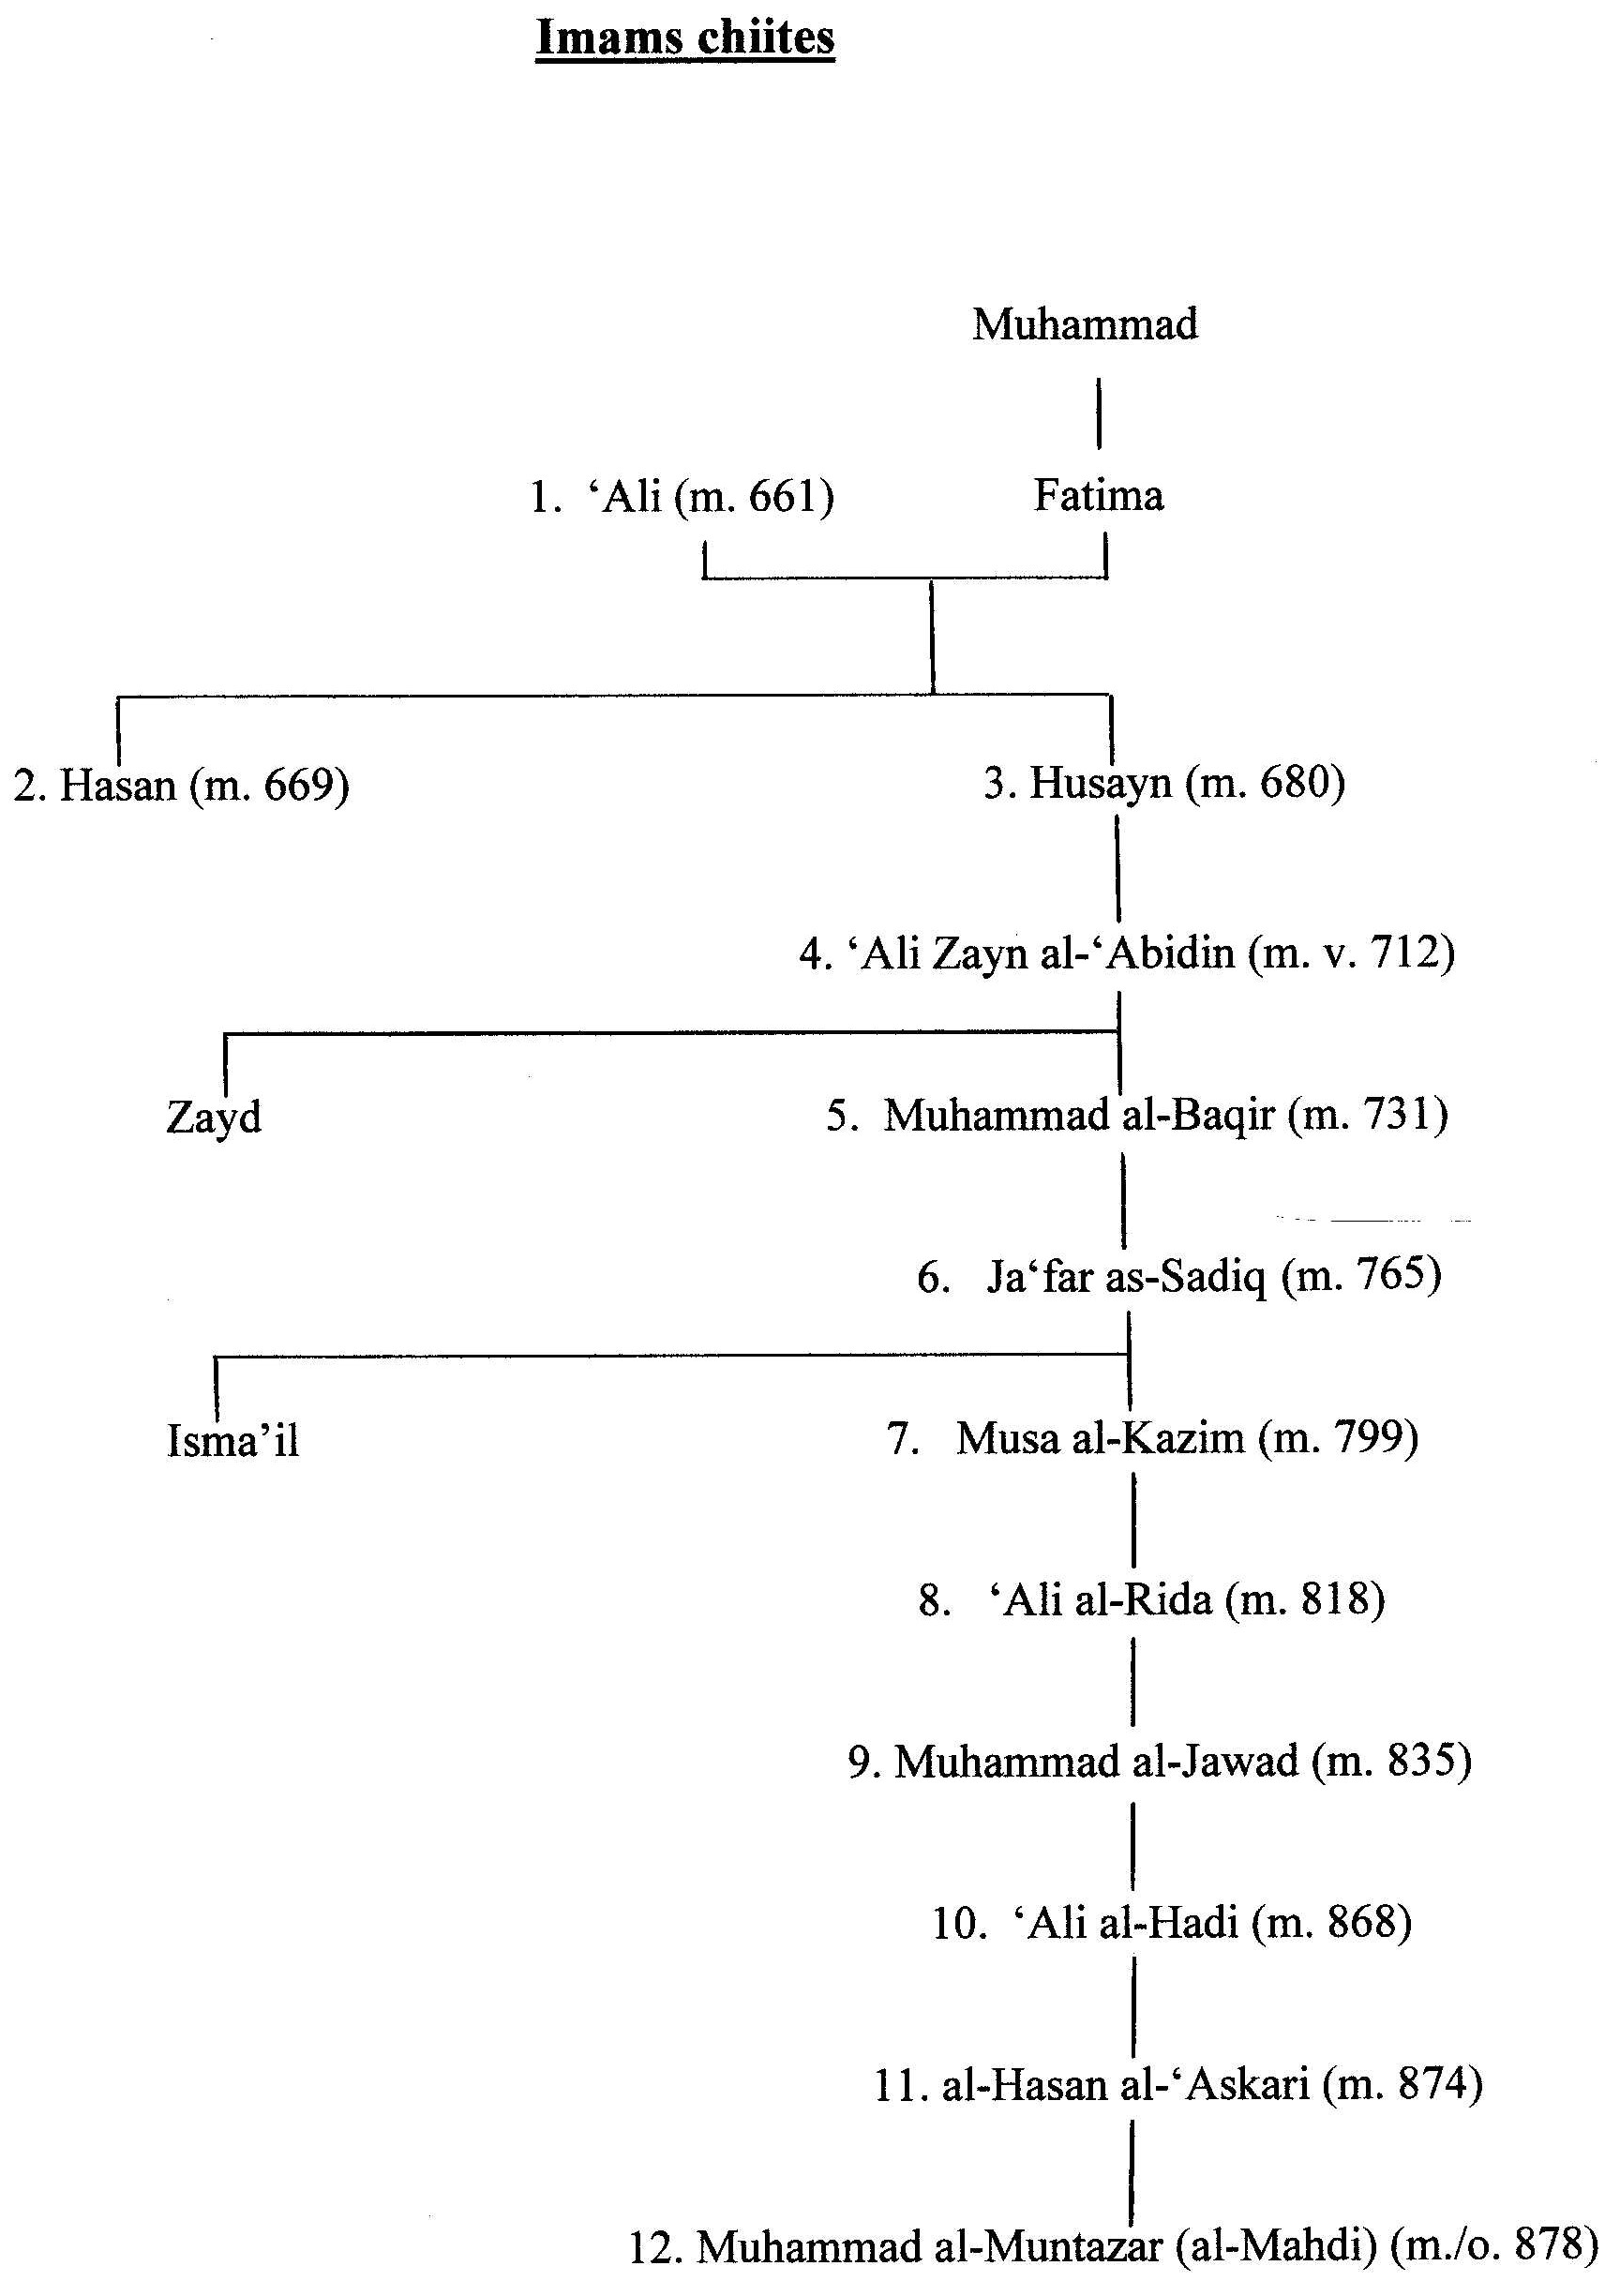
\includegraphics[width=5.58437in,height=7.90823in]{Image/media/image2.png}
\end{quote}

\hypertarget{glossaire-5}{%
\subsection{\texorpdfstring{\underline{Glossaire}}{Glossaire}}\label{glossaire-5}}

\begin{quote}
\underline{Personnes} Abbas Abu Bakr

Adud ad-Dawla Al-Karaki Hasan as-Sabah Isma'il

Kulayni (\emph{Kitab al-Kafi}) Mu'awiya (omeyyades) Nizar

Omar Osman Quraysh Yazid

\underline{Lieux} Alamut Ardabil

Ghadir al-Khumm Jabal al-Amil Kerbala

Khorasan Kufa Machhad Sham Siffin

\underline{Autres noms propres} akhbari

ja`farisme (école juridique chiite) kharijites

Mamlouks

Muharram (mois musulman) mu`tazilites

nizayri Qarmates Seljukides usuli

\underline{Notions}

ahl al-bayt : \emph{famille du Prophète (Mahomet, Ali, Fatima, Hasan,
Hoseyn)}

baten : \emph{ésotérique} (c. zaher) faqih (pl. fuqaha) : \emph{juriste}

fitna: \emph{discorde, querelle (conflit interne au monde musulman)}

ghulat : \emph{groupes chiites aux doctrines}

\emph{« extrémistes »}

hulul : \emph{« incarnation »}

ijtihad : \emph{effort personnel d'interprétation (des textes sacrés)}

`ilm : \emph{science}

imamzade : \emph{descendant des Imams / sanctuaire contenant leur
tombeau} (persan)

`isma : \emph{impeccabilité}

mahdi : \emph{« le voilé » : l'homme mystérieux qui viendra annoncer et
provoquer la fin des temps (= dernier imam (occulté) pour les chiites).}

ma`sum : \emph{impeccable (sans péché)} mujtahid : \emph{celui qui
pratique l'ijtihad} najes : \emph{impur} (persan)

na'ib : \emph{délégué}

na'ib al-`amm : \emph{représentant général de l'Imam}

nass : \emph{élection divine}

tafsir : \emph{commentaire (exotérique) du Coran}

tanasukh : \emph{métempsychose}

ta'wil : \emph{herméneutique ésotérique du Coran} ta'ziyya :
\emph{représentation théâtrale du drame de Kerbala}

taqiyya : \emph{dissimulation (fait de cacher sa foi)} walayat al-faqih
(persan : velayat-e faqih) : \emph{gouvernement du juriste}

zaher : \emph{exotérique} (c. de baten)

\textbf{\underline{Quelques traditions chiites}}
\end{quote}

\begin{enumerate}
\def\labelenumi{\arabic{enumi}.}
\item
  \begin{quote}
  \underline{Le « Coran chiite »}
  \end{quote}
\end{enumerate}

\begin{quote}
Certains écrits chiites rapportent des citations du « Coran intégral »
qui aurait été par la suite altéré par les sunnites. Ces citations
présentent des divergences parfois notables avec la recension
officielle, comportant souvent des mots, expressions ou bouts de phrase
absents de celle-ci (en italique dans le texte).

C. 4, 167-70 : « Ceux qui sont injustes \emph{à l'égard des droits de la
Famille de Muhammad}, Dieu ne les pardonnera ni ne les guidera sur aucun
chemin si ce n'est sur celui de la géhenne où ils y séjourneront à
jamais et c'est chose facile à Dieu.

C. 16, 24 : « Et quand on leur dit : `\,`Qu'a fait descendre votre
Seigneur \emph{au sujet de `Ali} ?'\,' Ils répondent : `\,`Fables
racontées par les Anciens'\,' » ?

C. 33, 71 : « Quiconque obéit à Dieu et à Son prophète \emph{en ce qui
concerne la walaya de `Ali et la walaya des imams après lui}, celui-là
jouit d'un bonheur grandiose ».

C. 42, 13 : « Il a établi pour vous, \emph{ô famille de Muhammad}, en
fait de religion, ce qu'Il avait prescrit à Noé, et ce que Nous te
révélons \emph{ô Muhammad}, et ce que Nous avons prescrit à Abraham, à
Moïse et à Jésus : `\,`Etablissez la religion \emph{de la famille de
Muhammad}, ne vous divisez pas à son sujet et soyez unis ».

(Source : \emph{La religion discrète}, M.A Amir-Moezzi, Paris, Vrin,
2006, p. 179-180)
\end{quote}

\begin{enumerate}
\def\labelenumi{\arabic{enumi}.}
\setcounter{enumi}{1}
\item
  \begin{quote}
  \underline{La divinité des Imams}
  \end{quote}
\end{enumerate}

\begin{quote}
De nombreux hadiths des Imams soulignent leur caractère quasi-divin :

« Hommes ! Dieu créa Ses serviteurs afin que ceux-ci Le connaissent car
lorsqu'Ils le connaissent, ils L'adorent et se libèrent ainsi de
l'adoration de tout autre que Lui ». Un homme demande alors à l'imam : «
Qu'est-ce que la connaissance de Dieu ? » « C'est pour les gens de
chaque époque, la connaissance de l'imam {[}de cette époque{]} auquel
ils doivent obéissance » (Husayn ben `Ali)

« Dieu fit de nous Son œil parmi ses adorateurs, Sa Langue Parlante
parmi Ses créatures, Sa Main de bienveillance et de miséricorde étendue
au-dessus de Ses serviteurs, Sa face grâce à laquelle on se dirige vers
Lui, Son Seuil qui guide vers Lui, Son Trésor au ciel et sur la
terre\ldots C'est par notre acte d'adoration que Dieu est adoré, sans
nous, Dieu ne saurait être adoré » (Ja`far as-Sadiq)

(Source : « Remarques sur la divinité de l'Imam », M-A Amir-Moezzi,
\emph{Studia Iranica}, n° 25, 1996, p. 193-216)
\end{quote}

\begin{enumerate}
\def\labelenumi{\arabic{enumi}.}
\setcounter{enumi}{2}
\item
  \begin{quote}
  \underline{Prophétie et imamat}
  \end{quote}
\end{enumerate}

\begin{quote}
Une autre tradition savante rapporte :

« Deux mille ans avant la création, Muhammad et Ali étaient une lumière
devant Dieu -- qu'Il soit glorifié et exalté -, lumière formée d'un
tronc principal d'où partait un rayon de lumière resplendissant\ldots{}
Dieu dit alors : « Voici une lumière {[}tirée{]} de Ma propre Lumière ;
son tronc est la prophétie et sa branche, l'imamat ; la prophétie
revient à Muhammad, Mon serviteur et messager, et l'imamat revient à
Ali, ma Preuve et mon Ami. Sans eux, je n'aurai rien créé de ma
création\ldots{} C'est pourquoi Ali répétait toujours : « Je proviens de
Muhammad {[}ou de Ahmad{]} comme une clarté provenant d'une
autre\ldots{} »

(Source : \emph{La religion discrète}, M-A Amir Moezzi, Paris, Vrin,
2006, p. 110)

3. \underline{Le martyre de l'imam Husayn}

Dans ce contexte, le martyre de Husayn, 3\textsuperscript{ème} imam, est
interprété dans les termes d'un sacrifice cosmique :

Avant que le monde ne soit, Dieu rassembla les âmes des Quatorze
Immaculés, déjà créées, en une grande assemblée et leur annonça que,
pour ce monde qu'Il était sur le point de façonner, « du sang doit être
donné, un nourrisson et un tout jeune marié tués, une jeune femme
emprisonnée ». Aucun n'eut la force d'accepter de telles souffrances, ni
même Muhammad, ni Ali, ni Hasan. Seul Hoseyn se porta volontaire. Dieu
insista :
\end{quote}

\begin{itemize}
\item
  \begin{quote}
  Tu devras donner les tiens.
  \end{quote}
\item
  \begin{quote}
  J'accepte.
  \end{quote}
\item
  \begin{quote}
  Tu devras donner ta tête.
  \end{quote}
\item
  \begin{quote}
  J'accepte.
  \end{quote}
\item
  \begin{quote}
  Une partie de ta famille devra connaître l'exil et la détention.
  \end{quote}
\item
  \begin{quote}
  J'accepte.
  \end{quote}
\end{itemize}

\begin{quote}
Alors Gabriel lui donna à boire la coupe de la souffrance et lui fit
signer un pacte où étaient inscrites toutes ses promesses.

Bien plus tard, lors de sa vie terrestre, approcha le temps de son
sacrifice. Il se trouvait à Karbalâ, accompagné de 72 fidèles compagnons
et de toute sa famille, encerclé par les armées de Yazid. Une armée de
djinns vint alors proposer ses services mais Hoseyn refusa : le combat
aurait été trop inégal et il se rappelait par ailleurs sa promesse. La
lutte commença et de nombreux êtres chers à Hoseyn, compagnons, fils,
frères, cousins, tombèrent l'un après l'autre sous les coups de
l'ennemi. Aveuglé par la douleur, Hoseyn en oublia sa promesse, et se
mit à tailler en morceaux l'armée adverse. Dieu s'empressa alors
d'envoyer Gabriel lui tendre le pacte qu'il avait signé au début des
temps. Rappelé à la raison, Hoseyn se soumit à la volonté divine et tint
son serment ; il retira son épée du combat et se livra à la fureur de
ses adversaires qui ne tardèrent pas à le mettre en pièces.

(Source : tradition orale relevée par A-S Vivier-Muresan : \emph{Afzâd.
Ethnologie d'un village d'Iran}, Peeters, 2006, p. 48).

Les courants de l'islam contemporain (9)
\end{quote}

\begin{enumerate}
\def\labelenumi{\Roman{enumi}.}
\item ~
  \hypertarget{le-ruxe9formisme-chiite}{%
  \subsection{\texorpdfstring{\underline{Le réformisme
  chiite}}{Le réformisme chiite}}\label{le-ruxe9formisme-chiite}}

  \begin{enumerate}
  \def\labelenumii{\arabic{enumii}.}
  \item
    \begin{quote}
    Un mouvement parallèle au réformisme sunnite
    \end{quote}
  \item
    \begin{quote}
    Particularités du réformisme chiite : \emph{ijtihad, taqlid} et
    \emph{bid`a}
    \end{quote}
  \item
    \begin{quote}
    Réforme de la doctrine et des pratiques
    \end{quote}
  \end{enumerate}
\item ~
  \hypertarget{genuxe8se-et-destin-du-chiisme-politique-ruxe9volution-iranienne-et-ruxe9publique-islamique}{%
  \subsection{\texorpdfstring{\underline{Genèse et destin du chiisme
  politique : Révolution iranienne et République
  islamique}}{Genèse et destin du chiisme politique : Révolution iranienne et République islamique}}\label{genuxe8se-et-destin-du-chiisme-politique-ruxe9volution-iranienne-et-ruxe9publique-islamique}}

  \begin{enumerate}
  \def\labelenumii{\arabic{enumii}.}
  \item
    \begin{quote}
    Un contexte bien particulier : l'Iran pahlavi
    \end{quote}
  \item
    \begin{quote}
    Ruhollah Khomeyni (1902-1989) et le \emph{velâyat-e faqih}
    \end{quote}
  \item
    \begin{quote}
    `Ali Shariati (1933-1977) et la naissance du chiisme révolutionnaire
    \end{quote}
  \item
    \begin{quote}
    La République islamique
    \end{quote}
  \end{enumerate}
\end{enumerate}

\hypertarget{glossaire-6}{%
\subsection{\texorpdfstring{\underline{Glossaire}}{Glossaire}}\label{glossaire-6}}

\begin{quote}
\underline{Personnes}

Al-Amin (Muhsin)

Baqir al-Sadr (Muhammad) Borujerdi

Khameney Khatami

Khomeyni (Ruhollah) Mohammed Reza Shah Shariati (`Ali)

\underline{Lieux} Jabal Amil Karbala Najaf

Neauphle-le-Château

\underline{Notions}

ayatollah : « \emph{signe de Dieu » (sur terre) ; grade supérieur dans
le clergé chiite}. marja'-ye taqlid : \emph{« source d'imitation » ;
plus haut grade dans le clergé chiite.} tajdid : \emph{renouvellement}.

tawhid : \emph{unicité (divine).}

mujtahid : \emph{celui qui pratique l'ijtihad.}

musta`zafin : \emph{les opprimés.}

taghut : \emph{idole ; tyran}.

\textbf{Le \emph{velayat-e faqih} : Ruhollah Khomeyni (1902-1989)}

\emph{Méthode du gouvernement islamique. Ses différences avec les autres
gouvernements.}

Le gouvernement islamique ne ressemble à aucun autre gouvernement
actuellement en vigueur. Il n'est pas despotique. Le chef de l'État
n'est pas un despote qui se joue des biens et de la vie du peuple et en
fait ce qu'il désire, qui tue celui qu'il veut, et enrichit ou ennoblit
qui il veut, distribuant de-ci de-là les terres et les biens du peuple.
Le Prophète, Ali et les califes n'avaient pas ce genre d'attributions.
Le gouvernement islamique n'est ni despotique ni absolutiste, il est
constitutionnel, bien entendu pas au sens habituel du terme, où les lois
sont approuvées par des personnes et une majorité : constitutionnel, au
sens où les dirigeants sont tenus à un ensemble de « conditions »
définies dans le Coran et dans la Sunna du Prophète à la fois en ce qui
concerne l'exécutif et l'administration. Ces conditions ne sont rien
d'autre que les lois islamiques, celles-là mêmes qui doivent être
observées et appliquées. De cette manière, le gouvernement islamique est
le gouvernement de la Loi divine sur le peuple.

C'est ce qui constitue la différence fondamentale entre le gouvernement
islamique et les autre gouvernements constitutionnels, monarchiques et
républicains ; un autre fait capital est que dans ces régimes, les élus
du peuple ou le monarque sont les législateurs, tandis que dans l'Islam,
le seul législateur est Dieu, le Législateur sacré.

Personne n'a le droit d'émettre des lois, et aucune loi n'est applicable
si ce n'est celles du Législateur. Voilà pourquoi dans le gouvernement
islamique, au lieu de l'assemblée législative qui représente
habituellement l'un des trois pouvoirs, il existe une assemblée de
planification qui a pour rôle d'organiser les divers ministères au
regard des lois islamiques et de déterminer, à l'aide de ces plans et
sur tout le territoire, la manière d'accomplir les services publics.

L'ensemble des lois islamiques réunies dans le Coran et dans la Sunna
ont été acceptées par les musulmans et ceux-ci leur obéissent. Ceci
facilite la tâche du gouvernement qui devient du même coup le
coordinateur du peuple. Tandis que dans les autres régimes
constitutionnels, la majorité de ceux qui se font passer pour les
représentants de la majorité du peuple approuvent ce qui leur plaît au
nom de la loi, et ensuite s'imposent au peuple tout entier.

Le gouvernement de l'Islam est le gouvernement de la Loi. Dans cette
méthode de gouverne- ment, la souveraineté revient exclusivement à Dieu,
et la Loi constitue l'ordre et le décret de Dieu. La Loi de l'Islam,
Ordre de Dieu, règne d'une façon absolue sur tous et sur l'État islami-
que. Tout les hommes depuis le Prophète, jusqu'à ses califes et au
commun des mortels, sont définitivement soumis à la Loi, loi qui est
envoyée par Dieu et expliquée dans le Coran et par le Prophète. Si
celui-ci a pris la charge du califat, ce fut sur l'ordre de Dieu. Il est
Calife de Dieu sur terre et non pas calife sur sa propre initiative dans
l'intention de devenir le chef des musulmans. Lorsque des risques de
conflits se firent jour dans la communauté, étant donné le caractère
récent des conversions à l'Islam, Dieu s'est révélé au Prophète et l'a
engagé à annoncer le califat de toute urgence, ainsi, en plein désert.
Mahomet désigna alors Ali comme Calife en obéissant à la Loi, non pas
parce que celui-ci était son gendre ou qu'il avait rendu des services,
mais parce que lui-même en avait reçu la mission divine et qu'il
s'inclinait devant l'ordre divin. Dans l'Islam, le gouvernement signifie
l'obéissance à la Loi, et seule la Loi exerce son autorité sur la
société. Là où une certaine limitation des attributions a été donnée au
Prophète et aux Imams, c'est l'œuvre de Dieu. Chaque fois que le
Prophète a exprimé quelque chose ou annoncé une loi, c'était en
obéissance à la Loi divine, Loi à laquelle tout le monde sans excep-
tion doit obéir, le gouvernant comme le gouverné. Obéir au Prophète est
également un ordre de Dieu qui dit : « Obéissez au Prophète. » La
soumission aux responsables du gouvernement ou imams est également un
ordre de Dieu qui dit: «Obéissez aux Imans qui sont issus de vous. »

L'opinion des personnes, fût-ce celle du Prophète, n'a pas de prise sur
la Loi divine. Tous se plient à la volonté de Dieu. {[}\ldots{]}

\emph{L'Exercice du pouvoir du faqih, par les textes}

\emph{Les faqih justes, véritables successeurs des prophètes}

Dans l'un des \emph{ravâyat} les plus authentiques, il est dit : « Ali
rapporte les paroles du Prophète : Dieu ! Pardonne à mes successeurs.
(\emph{Il a répété cette parole trois fois}.) --- Qui sont tes
successeurs ?, lui a-t-on demandé. --- Ceux qui viendront après moi et
qui citeront et enseigneront au peuple mes hadith et ma Sunna. »

Par conséquent, il ne fait aucun doute que ce \emph{ravâyat} ne concerne
pas les rapporteurs de hadith, c'est-à-dire ceux qui les rédigent ; en
effet, un écrivain ne peut être calife du Prophète.

Il faut entendre par le mot calife qui est employé dans ce
\emph{ravâyat}, le \emph{faqih} de l'Islam. La diffusion des lois et
l'éducation du peuple seront à la charge des \emph{faqih} justes, car
s'ils ne le sont pas, ils ressembleront aux juges qui ont inventé des
\emph{ravâyat} contre l'Islam à la manière de Samarat Ebn-e-Djandâb.
S'il n'y a pas de \emph{faqih}, le peuple ne pourra pas connaître le
\emph{feqh}, la Loi de l'Islam. Alors deviendra possible la propagation
de milliers de \emph{ravâyat} fabriqués par les agents des oppresseurs
et les \emph{âkhond} courtisans, destinés à faire l'apologie des
sultans. {[}\ldots{]}

\emph{Les pleins pouvoirs des faqih}

Par conséquent, « les faqih sont les confidents des prophètes »,
signifie que les \emph{faqih} ont le droit de prendre en charge tout ce
qui était du domaine des prophètes. Comme ceux-ci, ce sont des hommes
qui ne doivent dévier d'aucune loi et qui sont purs et désintéressés des
biens de ce monde, comme il est dit à la fin du hadith cité plus haut :
« Tant qu'ils n'entrent pas dans le monde » (dans le bourbier de la
recherche des biens matériels !). Si donc un \emph{faqih} pense aux
biens terrestres, ce n'est pas un \emph{faqih} juste, et il n'est pas le
confident du Prophète, ni l'exécutant des lois islamiques. Seul le
\emph{faqih} juste est en mesure d'appliquer les Lois, d'établir les
principes islamiques, d'administrer les peines et les châtiments, de
veiller aux frontières et à l'intégrité territoriale de la communauté
musulmane, bref d'être le Magistrat suprême du gouvernement. Comme le
Prophète, il peut établir les principes islamiques et appliquer les
lois. {[}\ldots{]}

Extraits de \emph{Pour un gouvernement islamique}, 1969 (traduction
française chez Fayolle, 1979).
\end{quote}

\hypertarget{institutions}{%
\subsection{Institutions}\label{institutions}}

\begin{quote}
\textbf{De la République islamique d'Iran}
\end{quote}

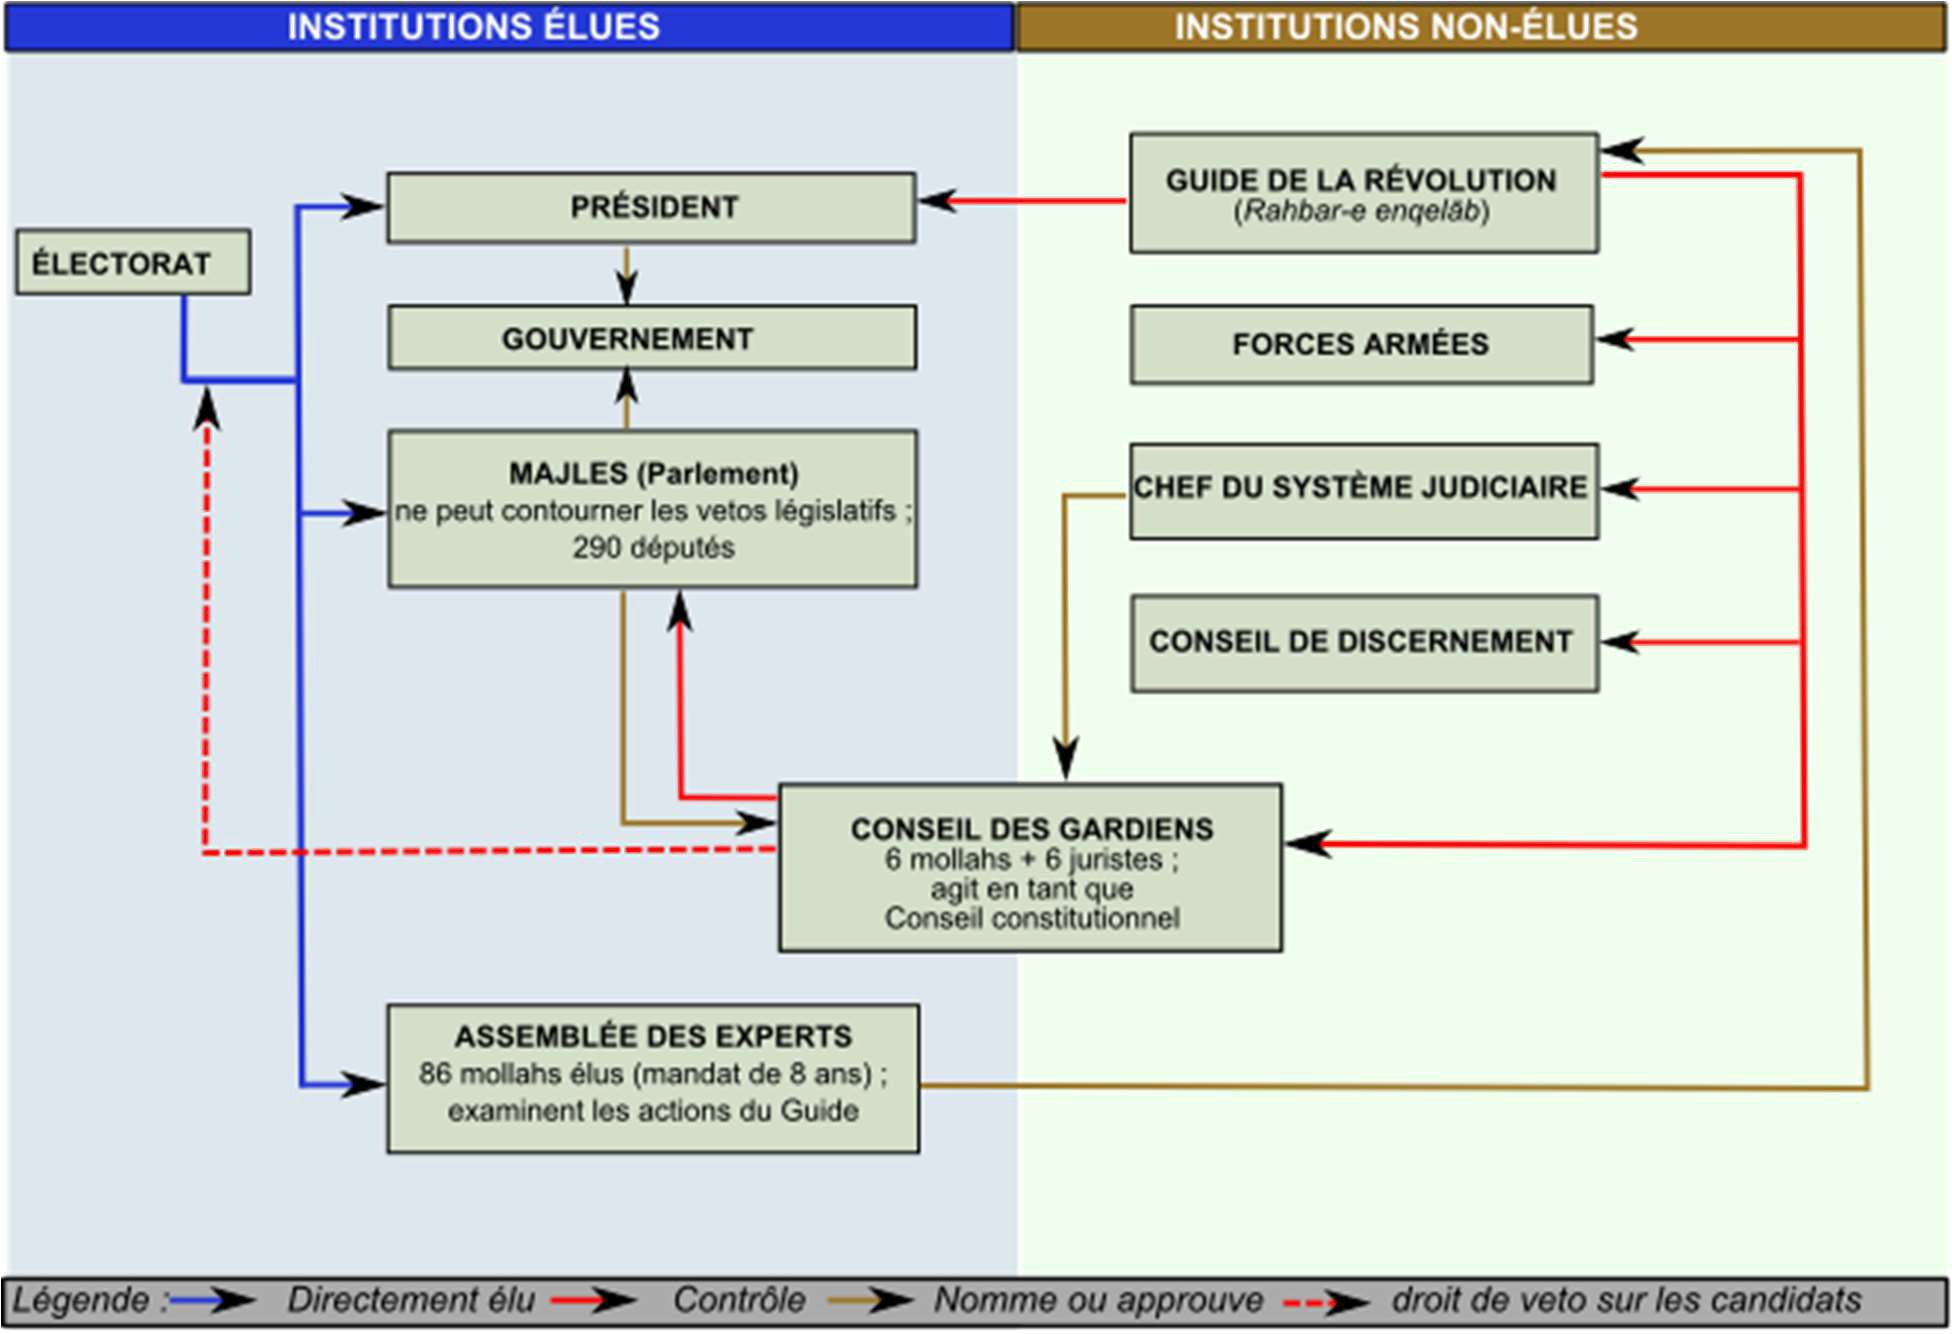
\includegraphics[width=6.30333in,height=4.30771in]{Image/media/image3.jpeg}

\begin{quote}
Les courants de l'islam contemporain (10)
\end{quote}

\begin{enumerate}
\def\labelenumi{\Roman{enumi}.}
\item ~
  \hypertarget{les-nouveaux-penseurs-essai-de-pruxe9sentation}{%
  \subsection{\texorpdfstring{ \underline{Les nouveaux penseurs : essai
  de
  présentation}}{ Les nouveaux penseurs : essai de présentation}}\label{les-nouveaux-penseurs-essai-de-pruxe9sentation}}

  \begin{enumerate}
  \def\labelenumii{\arabic{enumii}.}
  \item
    \begin{quote}
    Convergence certaine\ldots{}
    \end{quote}
  \item
    \begin{quote}
    \ldots Et diversité
    \end{quote}
  \end{enumerate}
\item ~
  \hypertarget{nouvelles-approches-critiques}{%
  \subsection{\texorpdfstring{ \underline{Nouvelles approches
  critiques}}{ Nouvelles approches critiques}}\label{nouvelles-approches-critiques}}

  \begin{enumerate}
  \def\labelenumii{\arabic{enumii}.}
  \item
    \begin{quote}
    L'approche littéraire
    \end{quote}
  \item
    \begin{quote}
    La critique historique
    \end{quote}
  \end{enumerate}
\item ~
  \hypertarget{le-statut-de-la-parole-de-dieu-un-coran-cruxe9uxe9}{%
  \subsection{\texorpdfstring{\underline{Le statut de la Parole de Dieu
  : un Coran créé
  ?}}{Le statut de la Parole de Dieu : un Coran créé ?}}\label{le-statut-de-la-parole-de-dieu-un-coran-cruxe9uxe9}}

  \begin{enumerate}
  \def\labelenumii{\arabic{enumii}.}
  \item
    \begin{quote}
    Le statut du Prophète
    \end{quote}
  \item
    \begin{quote}
    L' « abaissement » de la Parole
    \end{quote}
  \end{enumerate}
\item ~
  \hypertarget{la-question-de-linterpruxe9tation}{%
  \subsection{\texorpdfstring{\underline{La question de
  l'interprétation}}{La question de l'interprétation}}\label{la-question-de-linterpruxe9tation}}

  \begin{enumerate}
  \def\labelenumii{\arabic{enumii}.}
  \item
    \begin{quote}
    Approche littéraire
    \end{quote}
  \item
    \begin{quote}
    Approche scientifique
    \end{quote}
  \end{enumerate}
\end{enumerate}

\hypertarget{glossaire-7}{%
\subsection{\texorpdfstring{\underline{Glossaire}}{Glossaire}}\label{glossaire-7}}

\begin{quote}
\underline{Personnes}

Abu Zayd (Nasr Hamid) Al-Khuli (Amin) Arkoun (Mohamed) Charfi
(Abdelmajid) Engineer (Ali)

Esack (Farid) Hossein (Taha) Iqbal (Muhammad)

Khalafallah (Muhammad Ahmad) Rahman (Fazlur)

Shabestari (Muhammad) Sorush (Abdelkarim)

\underline{Notions}

tafsir : \emph{commentaire (exotérique) du Coran}

ta'wil : \emph{herméneutique ésotérique du Coran}
\end{quote}

\hypertarget{fazlur-rahman-1919-1988}{%
\subsection{\texorpdfstring{\underline{Fazlur Rahman
(1919-1988)}}{Fazlur Rahman (1919-1988)}}\label{fazlur-rahman-1919-1988}}

\begin{quote}
Pour le Coran lui-même, et par conséquent pour les Musulmans, le Coran
est la Parole de Dieu (kalâm Allâh). Mohammed, lui aussi, était
absolument convaincu de recevoir le Message de Dieu, le Tout-Autre (nous
essaierons plus loin de comprendre plus précisément le sens de cette
Altérité absolue), à tel point qu'il s'est basé sur la force de cette
conviction pour rejeter quelques-unes des assertions historiques les
plus fondamentales de la tradition Judéo-Chrétienne concernant Abraham
et les autres Prophètes. Cet "Autre", par un certain canal, a "dicté" le
Coran avec une autorité absolue. La voix surgissant des profondeurs de
la vie parlait distinctement, impérieusement, sans méprise possible. Non
seulement le mot \textbf{"}\emph{qur'ân}", signifiant "récitation",
l'indique clairement, mais le texte du Coran lui-même déclare en
plusieurs endroits que le Coran est révélé verbalement et non pas
seulement son "sens" et ses idées. Le terme coranique pour "Révélation"
est \emph{wahy} dont le sens est assez proche d' "inspiration", à
condition que ce mot ne soit pas censé exclure nécessairement le mode
verbal (par "Parole", bien entendu, nous ne voulons pas dire le Son). Le
Coran dit: "Dieu ne parle à aucun humain (c'est-à-dire en paroles
audibles) excepté par \emph{wahy} (c'est-à-dire par idée-parole,
inspiration) ou derrière un voile, ou bien Il envoie un Messager (un
ange) qui parle par \emph{wahy}...Nous t'avons ainsi révélé un Esprit
qui est à nos ordres". (Q. 42,51-52)

Pendant le 2° et le 3° siècles de l'ère islamique, cependant, de
violentes différences d'opinion, des controverses, en partie causées par
l'influence des doctrines chrétiennes, s'élevèrent parmi les Musulmans
au sujet de la nature de la Révélation. L'"orthodoxie" islamique
émergente qui en était au point crucial de formuler son contenu précis,
mit alors l'accent sur l'origine externe de la Révélation Prophétique
afin d'en sauvegarder son "Altérité", son "Objectivité" et son caractère
verbal. Le Coran lui-même maintenait certainement son altérité vis-à-vis
du Prophète. Il déclare en effet: "\emph{L'Esprit fidèle l'a fait
descendre sur ton coeur pour que tu sois au nombre des avertisseurs}"
(Q. 26,194), et encore: "\emph{Dis: Qui est l'ennemi de Gabriel (qu'il
le soit), car c'est lui qui a fait descendre sur ton coeur... le Livre}"
(Q. 2,97). Mais il manquait à l'orthodoxie (en fait, à toute la pensée
médiévale) d'avoir les instruments intellectuels nécessaires pour
allier, dans sa formulation du dogme, l'Altérité et le caractère verbal
de la Révélation d'une part, et, d'autre part, son lien intime avec
l'oeuvre et la personnalité religieuse du Prophète, c'est-à-dire qu'il
lui manquait la capacité intellectuelle de dire, à la fois, que le Coran
est entièrement la Parole de Dieu et aussi, dans un sens ordinaire, la
parole de Mohammed. Le Coran affirme clairement les deux idées, car s'il
insiste sur le fait qu'il est descendu sur le "coeur" du Prophète,
comment peut-il lui être extérieur ? Ceci, bien sûr, n'implique pas
nécessairement que le Prophète ne percevait pas un personnage extérieur,
comme la tradition le dit, mais il est remarquable que le Coran lui-même
ne fait aucune mention d'un personnage dans ce contexte: ce n'est qu'en
lien avec certaines expériences (habituellement liées à l'Ascension du
Prophète), que le Coran parle du prophète comme de quelqu'un ayant vu un
personnage ou un esprit ou quelque autre objet "à la lointaine limite"
ou "à l'horizon" bien qu'ici encore, comme nous l'avons dit,
l'expérience soit décrite comme étant d'ordre spirituel. Mais
l'orthodoxie, par les \emph{hadith} ou les "traditions" transmises du
Prophète, en partie interprétées correctement, et en partie inventées,
ainsi que par une discipline théologique largement basée sur le
\emph{hadith}, fit de la Révélation prophétique un phénomène ne frappant
que son oreille, uniquement extérieur à lui, considérant l'ange ou
"l'esprit qui vient sur le cœur" comme un agent totalement externe.
L'image que l'Occident moderne garde de la Révélation prophétique se
base largement sur cette formulation orthodoxe plutôt que sur le Coran,
d'ailleurs la foi du Musulman ordinaire fait de même.

... Lorsque la perception intuitive de la morale chez Mohammed atteint
son plus haut point et s'identifie avec la morale elle-même, la Parole
est donnée avec l'inspiration elle-même. Le Coran est donc la pure
Parole divine, mais évidemment, il est également relié intimement à la
personnalité interne du Prophète Mohammed, dont la relation au Coran ne
peut être conçue mécaniquement comme un disque enregistré. La Parole
divine passe par le cœur du Prophète.

\emph{Extrait de son livre \textbf{Islam} (Doubleday Anchor Book, New
York, 1968, 331 pp.), p. 25-28.}

Les courants de l'islam contemporain (11)
\end{quote}

\begin{enumerate}
\def\labelenumi{\Roman{enumi}.}
\item ~
  \hypertarget{duxe9finitions}{%
  \subsection{\texorpdfstring{
  \underline{Définitions}}{ Définitions}}\label{duxe9finitions}}

  \begin{enumerate}
  \def\labelenumii{\arabic{enumii}.}
  \item
    La \emph{shari`a}
  \item
    \begin{quote}
    Le \emph{fiqh}
    \end{quote}
  \end{enumerate}
\item ~
  \hypertarget{l-amuxe9nagement-du-droit}{%
  \subsection{\texorpdfstring{\underline{L' « aménagement » du
  droit}}{L' « aménagement » du droit}}\label{l-amuxe9nagement-du-droit}}

  \begin{enumerate}
  \def\labelenumii{\arabic{enumii}.}
  \item
    \begin{quote}
    Méthode et principes
    \end{quote}
  \item
    \begin{quote}
    La question des \emph{fatwa}
    \end{quote}
  \item
    \begin{quote}
    L'enjeu des musulmans d'Occident et le « \emph{fiqh} des minorités »
    \end{quote}
  \end{enumerate}
\item ~
  \hypertarget{repenser-la-norme}{%
  \subsection{\texorpdfstring{\underline{Repenser la
  norme}}{Repenser la norme}}\label{repenser-la-norme}}

  \begin{enumerate}
  \def\labelenumii{\arabic{enumii}.}
  \item
    \begin{quote}
    Le dynamisme de la \emph{shari`a}
    \end{quote}
  \item
    \begin{quote}
    La \emph{shari`a} sans le \emph{fiqh ?}
    \end{quote}
  \end{enumerate}
\end{enumerate}

\begin{quote}
\textbf{\underline{Glossaire}}

\underline{Personnes}

Al-Qaradawi (Sheikh Yusef) Charfi (Abdelmajid)

Oubrou (Tareq) Rahman (Fazlur) Ramadan (Tariq) Talbi (Mohammed)

\underline{Notions}

dar ash-shahadat : \emph{« maison » (terre) du témoignage}

dar al-da`wa : \emph{« maison » (terre) du témoignage}

fatwa : \emph{opinion sur un point de la loi islamique donnée par un}
mufti\emph{.} furu' al-fiqh : \emph{« branches » du droit (discipline
juridique)}

haqq allah : \emph{droit de Dieu}

haqq al-nas : \emph{droit des gens}

`ibadat : \emph{culte/partie du droit concernant le culte.}

ijma' : \emph{consensus (des juristes, de la communauté).}

\underline{Lieux}

Al-Azhar (Egypte) Qarawiya (Maroc) Zaytuna (Tunisie)

maqasid : \emph{intention, finalité} mu`amalat : \emph{relations/partie
du droit concernant les relations humaines.} naskh : \emph{abrogation}

shari`at allah : \emph{« voie » de Dieu} shari'at al-Masih:
``\emph{voie'' du Christ (= religion chrétienne)}

shari'at Musa: \emph{``voie'' de Moïse (= religion juive)}

talfiq : \emph{éclectisme (fait de choisir librement entre les
différentes écoles juridiques)}

usul al-fiqh : \emph{fondements du droit (discipline juridique)}
\end{quote}

\hypertarget{tareq-oubrou}{%
\subsection{\texorpdfstring{\underline{Tareq
Oubrou}}{Tareq Oubrou}}\label{tareq-oubrou}}

\begin{quote}
\textbf{L'islam est-il une religion de la loi ?}

TAREQ OUBROU : Il y a une autre catégorie d'intellectuels qui pousse le
raisonnement plus loin en considérant que le Coran n'est ni juridique ni
éthique, mais seulement spirituel (car pour eux, même l'éthique est
contraignante).

LEÏLA BABES : Quels intellectuels ? Pouvez-vous citer des noms ?

TAREQ OUBROU : Peu importe les noms. C'est tellement répandu aujourd'hui
chez les musulmans que la foi c'est dans le cœur, dans le sens de la
libération par rapport aux normes rituelles et éthiques. Mais on oublie
qu'une foi qui demeure dans le cœur, qui ne s'exprime pas à travers un
comportement éthique et spirituel cultuel, risque d'étouffer et de
s'éteindre.

Pour eux, le Coran est un message de foi uniquement, presque une forme
de protestantisme poussé à l'extrême. Car lorsqu'il a commandé d'oeuvrer
pour le bien et de prévenir le mal, il n'a pas désigné de quel bien ou
de quel mal il s'agit ni comment réaliser tout cela. Et si l'on suit
cette démarche, on aboutira à la question suivante : y a-t-il une
éthique musulmane ? N'y a-t-il pas une morale universelle, et pourquoi
alors la chercher dans les Sources révélées ? Même le rite n'échappera
pas à de telles interrogations à un moment donné. Par exemple, ni le
nombre ni la forme des prières canoniques, deuxième pilier de l'islam,
ne sont cités dans le Coran. Puisque la prière est très contraignante,
certainement la plus contraignante pour beaucoup, voire pour la majorité
des musulmans, doit-on pour cela l'effacer et la transformer en une
notion allégorique, et donc à chacun sa prière, et on aurait autant
d'islams que de musulmans ? On tombe finalement dans un mysticisme
obscur.

Mais tant qu'on n'a pas compris que le Coran sans la Sunna du Prophète
reste illisible, et qu'il y a des règles d'interprétation issues de ces
mêmes sources, on suivra un enchaînement de questionnements pour aboutir
à l'annihilation pure et simple des valeurs de l'islam. Trouver la loi
contraignante ne doit pas aller jusqu'à abolir des références et des
normes, ce qui plongerait les musulmans encore plus dans le chaos.

Extrait du livre \emph{Loi d'Allah, loi des hommes} de T. Oubrou et L.
Babès, Albin Michel, Paris, 2002, p. 86-87.
\end{quote}

\hypertarget{lhuxe9ritage-fuxe9minin}{%
\subsection{L'héritage féminin}\label{lhuxe9ritage-fuxe9minin}}

\begin{quote}
Vous avez évoqué l'héritage de la femme qui est la moitié de celui de
l'homme. Il faut signaler que le droit successoral en islam a répondu à
des milliers de cas. La règle de la moitié de l'homme donnée à la femme
n'est pas valable pour tous les cas. Nous avons le verset qui donne dans
un cas précis un sixième à la femme et un sixième à l'homme (IV, 11-12).
L'homme qui hérite le double de sa sœur doit subvenir aux besoins de sa
famille, ce qui n'est pas un devoir pour la femme ; ce qu'elle hérite va
dans sa poche, elle peut le faire fructifier, créer une entreprise sans
la permission ni de son frère, ni de son père, ni de son mari, etc. (et,
comme vous le savez bien, la femme en droit musulman est indépendante
économiquement de son mari dans le sens où, s'il subit une faillite, ses
biens restent protégés). Elle exigera de son mari une garantie
matérielle, qu'elle définit. En plus, les femmes ont inventé leur « ruse
» : une partie de la dot est effectivement versée au début du mariage,
l'autre ne devient exigible qu'en cas de divorce... mais cette part
conditionnelle est très élevée.

Ces fictions juridiques (\emph{hiyal}), qui existent dans tous les
systèmes juridiques du monde, permettent de préserver l'esprit de la
shari`a et de remédier aux abus possibles. La femme peut donner la
\emph{zakat} (aumône légale, quatrième pilier de l'islam) --- considérée
comme des restes --- à son mari, ce qui n'est pas permis dans l'autre
sens ; il n'a pas à lui donner de ses restes, tout en sachant que les
biens de sa femme restent intouchables. Elle ne donne pas de
\emph{zakat} sur ses bijoux même si elle en a une tonne... Le juge peut
divorcer le mari si celle-ci porte plainte à cause de son manquement à
ses devoirs matériels.

Il serait donc injuste dans un tel système de donner la même part à la
sœur et au frère. Il y aura toujours mille dispositions juridiques dans
le droit musulman pour garantir l'esprit d'équité, qui

est tout sauf statique. Revenons à ce concept de l'éthicisation, il me
permet d'avancer que si la moitié donnée à la fille dans certaines
conditions lui cause une réelle injustice, la part ajoutée par un
testament peut y remédier. En effet le seul hadith qui interdit le
testament à un héritier désigné par les textes est discutable. Il ne
fait pas l'unanimité chez les traditionnistes critiques. L'énoncé du
hadith est : « Pas de testament pour un héritier légitime. » Les
héritiers légitimes sont ceux qui sont indiqués par le Coran et la Sunna
ou étendus par analogie. Ce hadith rapporté par Nassây (m. en 1277),
Tirmidhi (m. en 892), Abu Dawûd (m. en 888) et Ahmed, ne résiste pas aux
scalpels des traditionnistes critiques. C'est pourquoi Bukhâri ne l'a
pas rapporté dans son Sahîh, car il n'est pas authentique selon ses
règles. Muslim non plus ne l'a pas rapporté. Il existe une autre version
qui dit : « Pas de testament à celui qui hérite légalement sauf si les
autres héritiers consentent », sans toutefois dépasser le tiers de
l'ensemble de la succession ; certains n'ont pas établi de limites. Je
suis de l'avis de Al-Mahdi Al-Murtada qui me permet de stipuler que le
testament pour la fille en plus de sa moitié est possible. Et je vois en
ce sujet que l'abrogation du testament ne signifie pas l'abrogation de
sa permission, mais celle de son imposition qui était obligatoire.
L'imam Shafi'i avance l'\emph{ijmâ'} en cette matière mais je ne vois
pas la base sur laquelle il est fondé. Il ne pouvait pas avancer
l'abrogation par ce hadith, il n'y a pas d'abrogation d'un verset par un
hadith, avis que je

partage.

L'une des raisons légales qui me permettent cet avis est que la
situation financière des filles sous l'effet de l'éclatement des liens
familiaux a bien changé. Elle a acquis une plus grande indépendance
économique, et c'est elle qui prend dans beaucoup de cas la charge de
toute une famille. Dans ces conditions et par le biais du « testament
obligatoire », l'on peut élever la part de la sœur jusqu'à égalité de
celle du frère. C'est à traiter au cas par cas en fonction de la
jurisprudence.

Donc si j'ai évoqué l'intégration des coutumes, mais aussi des
mentalités et des conventions sociales dans le droit islamique, ce n'est
pas pour perpétuer les injustices mais justement pour les lever. Et s'il
y a une mauvaise application de droit musulman en matière d'héritage,
c'est pour une simple raison : l'éclatement des sociétés musulmanes.
C'est pourquoi j'ai parlé de l'éthicisation de la shari'a qui consiste à
moduler l'application du droit sur des bases morales en gardant
justement en vue les grands principes d'équité.

Extrait du livre \emph{Loi d'Allah, loi des hommes} de T. Oubrou et L.
Babès, Albin Michel, Paris, 2002, p. 103-105.
\end{quote}

\hypertarget{mohammed-talbi}{%
\subsection{\texorpdfstring{\underline{Mohammed
Talbi}}{Mohammed Talbi}}\label{mohammed-talbi}}

\begin{quote}
\textbf{L'héritage féminin}

\emph{Pourquoi la question de l'héritage pose-t-elle tant problème, y
compris en Tunisie qui a pourtant fait des efforts considérables pour
moderniser le droit de la famille ?}

C'est le seul problème vraiment délicat. En matière sexuelle, l'islam
est en effet très libéral puisqu'il admet même une certaine forme de
prostitution avec le mariage \emph{mut'a}. Ce libéralisme a d'ailleurs
constitué au Moyen Age un des points forts de la polémique chrétienne
contre l'islam, considéré comme trop laxiste et permissif. Aujourd'hui,
c'est l'inverse. Le problème de l'héritage n'est pas, cela dit,
totalement insoluble. D'abord parce qu'on peut doter les filles de son
vivant pour rétablir l'équilibre. Beaucoup de parents le font déjà. A
plus long terme, si les femmes parviennent à s'imposer davantage dans la
société et à faire aboutir leurs revendications, car les hommes ne leur
feront pas de cadeaux, rien ne dit qu'on n'aboutira pas un jour à un
consensus qui trouverait une solution juridique conforme à l'islam.
L'orientation du Coran va, je vous l'ai dit, dans le sens de
l'émancipation des femmes, telle est la finalité de la révélation. On
peut donc dire que la femme est parvenue aujourd'hui à un haut degré de
maturité, que la conjoncture sociale a changé, qu'elle travaille etc.,
ce qui permet de lui concéder la parité totale avec l'homme. Il existe
trois principes en islam permettant de faire évoluer le droit et de
l'adapter

à la réalité, la \emph{maslaha} c'est-à-dire l'utilité publique, un
concept qui date du II\textsuperscript{e} siècle de l'hégire, la
\emph{zharoura}, la nécessité, c'est un principe fort puisqu'il est dit
que "la nécessité rend permis l'interdit" ; et les \emph{maqassid}, les
finalités de la loi. Ces trois instruments permettent de faire évoluer
cette dernière, mais il faut que la société y soit préparée. Cela pas
été le cas jusqu'à présent. Le jour où cela arrivera, les musulmans
trouveront dans leur patrimoine les éléments nécessaires pour faire
évoluer la loi sans rupture avec la foi.

Extrait de son livre \emph{Un islam moderne}, Cérès, Tunis, 1998, p.
153-154.

Les courants de l'islam contemporain (12)
\end{quote}

\begin{enumerate}
\def\labelenumi{\Roman{enumi}.}
\item ~
  \hypertarget{un-siuxe8cle-difficile}{%
  \subsection{\texorpdfstring{\underline{Un siècle
  difficile}}{Un siècle difficile}}\label{un-siuxe8cle-difficile}}

  \begin{enumerate}
  \def\labelenumii{\arabic{enumii}.}
  \item
    \begin{quote}
    Facteurs politiques
    \end{quote}
  \item
    \begin{quote}
    Facteurs idéologiques et sociaux
    \end{quote}
  \end{enumerate}
\item ~
  \hypertarget{ruxe9sistance-et-renouveau}{%
  \subsection{\texorpdfstring{\underline{Résistance et
  renouveau}}{Résistance et renouveau}}\label{ruxe9sistance-et-renouveau}}

  \begin{enumerate}
  \def\labelenumii{\arabic{enumii}.}
  \item
    \begin{quote}
    Une fin de siècle plus clémente
    \end{quote}
  \item
    \begin{quote}
    Sur la voie de la modernité : les néo-confréries
    \end{quote}
  \end{enumerate}
\item ~
  \hypertarget{soufisme-fondamentalisme-modernisme-des-relations-complexes}{%
  \subsection{\texorpdfstring{\underline{Soufisme, fondamentalisme,
  modernisme : des relations
  complexes}}{Soufisme, fondamentalisme, modernisme : des relations complexes}}\label{soufisme-fondamentalisme-modernisme-des-relations-complexes}}

  \begin{enumerate}
  \def\labelenumii{\arabic{enumii}.}
  \item
    \begin{quote}
    Soufisme et fondamentalisme
    \end{quote}
  \end{enumerate}
\end{enumerate}

\begin{quote}
2. Confrérisme et modernisme : l'exemple des Fethullahci
\end{quote}

\begin{enumerate}
\def\labelenumi{\Roman{enumi}.}
\setcounter{enumi}{3}
\item ~
  \hypertarget{le-soufisme-en-occident}{%
  \subsection{\texorpdfstring{\underline{Le soufisme en
  Occident}}{Le soufisme en Occident}}\label{le-soufisme-en-occident}}

  \begin{enumerate}
  \def\labelenumii{\arabic{enumii}.}
  \item
    \begin{quote}
    Les origines : René Guénon
    \end{quote}
  \item
    \begin{quote}
    Du soufisme « immigré » au soufisme français
    \end{quote}
  \end{enumerate}
\end{enumerate}

\begin{quote}
\underline{Personnes}

Bentounès (Khaled) (1949 -) Guénon (René) (1884-1951) Gülen (Fethullah)
(1938 -)

Ilyas (Muhammad) (1885-1944) Naqshband (Baha'uddin) (m. 1388) Nursi
(Sa`id) (1873-1960)

Schuon (Frithjof) (1907-1998) Skali (Faouzi) (1953 -) Vâlsan (Michel)
(1907-1974) Yasawi (Ahmad) (m. 1166)

\underline{Confréries} `Alawiyya Bektashi Butshishiyya Haqqaniyya
Mevlevi Naqshbandiyya Qubaysiyya Sanusiyya Shadhiliya Shishtiyya
Tijaniyya
\end{quote}

\hypertarget{glossaire-8}{%
\subsection{\texorpdfstring{\hfill\break
\underline{Glossaire}}{ Glossaire}}\label{glossaire-8}}

\begin{quote}
\underline{Autres mouvements} Tablighi jama`at Nurcu

Fethullahci

\underline{Notions}

\emph{bay`a} : allégeance =\textgreater{} en contexte soufi, relation
d'allégeance liant les disciples au maître

\emph{chilla} : retraite (spirituelle)

\emph{da`wa} : « invitation » =\textgreater{} prédication, appel à
entrer dans l'islam

\emph{dhikr (zikr)} : « souvenir » : pratique soufie fondée sur la
répétition du nom de Dieu. \emph{ijaza} : « autorisation »
=\textgreater{} reconnaissance officielle du titre de \emph{shaykh}

\emph{khalifa} : « successeur », « vicaire » =\textgreater{} maître
confrérique (v. \emph{shaykh, pir})

\emph{mawled} (\emph{mouled}) : pèlerinage (annuel) à un tombeau de
saint

\emph{murid} : disciple

\emph{pir} : maître confrérique (v. \emph{shaykh, khalifa})
\emph{sheykh} : maître confrérique (v. \emph{khalifa, pir})
\emph{tariqa} : voie =\textgreater{} confrérie

\emph{tekke} : lieu de rencontre confrérique (v. \emph{zawiyya})
\emph{zawiyya} : lieu de rencontre confrérique (v. \emph{tekke})
\emph{wird} : oraison personnelle
\end{quote}

\hypertarget{une-nuxe9o-confruxe9rie-islamiste}{%
\subsection{\texorpdfstring{\underline{Une néo-confrérie « islamiste
»}}{Une néo-confrérie « islamiste »}}\label{une-nuxe9o-confruxe9rie-islamiste}}

\begin{quote}
Au Maroc, le cheikh Abdessalame Yassine fonde en 1981 une structure de
type confrérique, la \emph{Jamâ`a}, qui a pour vocation la \emph{da`wa},
comprise comme rappel de Dieu à l'ensemble de la société. Cette
\emph{da'wa} a une dimension politique marquée : à terme est visée « la
construction d'une entité politique islamique, qui préparera des
élections islamiques, une constitution islamique et un gouvernement
islamique ». Sa doctrine est exposée dans une œuvre publiée en 1982 :
\emph{Al minhâj al-nabawi} (La voie prophétique). Voici sa pensée
présentée par le chercher Youssef Belal.

Le projet politique d'A. Yassine est largement déterminé par l'idée
qu'il se fait du rapport des croyants à Dieu, c'est-à-dire
essentiellement le rapport mystique. Non seulement la place du cheikh
médiateur entre Dieu et les hommes est indispensable mais la
transcendance vécue lors des rites soufis, le sentiment d'élévation et
de rapprochement de Dieu doit être un sentiment présent à tous les
instants et dans tous les actes des hommes. La structure du livre est
révélatrice à cet égard. Consacrant l'essentiel de son ouvrage aux dix
séances (\emph{khisâl}) qui permettront à l'homme de revivifier sa foi,
A. Yassine reprend largement les thèmes soufis : \emph{al-suhba}
(compagnonnage), \emph{al-dhikr} (remémoration), \emph{al-sidq} (la
sincérité), \emph{al-badl} (le don), \emph{al-`ilm} (le savoir),
\emph{al-jihâd} (la lutte contre l'égo).

Mais il faut bien voir que la pensée d'A. Yassine se déploie constamment
sur le registre de l'éducation, \emph{tarbiyya} et de l'organisation,
\emph{tanzîm}. La tension est permanente entre une éducation soufie et
une action qui se veut révolutionnaire dans le monde.

(\ldots)

L'allégeance à A. Yassine {[}est{]} un acte vital pour les adeptes. Pour
suivre sa voie et son enseignement, il est indispensable de faire preuve
de \emph{sidq}, c'est-à-dire que l'adepte doit suivre tout ce que lui
prescrivent la Jamâ`a et son guide. Ceux qui veulent suivre la voie du
Prophète, c'est-à-dire la voie d'A. Yassine, doivent être conscients que
l'ego, le \emph{nafs}, peut être un obstacle à tout moment. Il faut
combattre le \emph{nafs} qui est le mal (\emph{su'}). Valoriser son
\emph{nafs} est en fait incompatible avec le rôle assigné à la Jamâ`a et
à A. Yassine. Il faut être capable de se dévouer pour la Jamâ'\,`a et
pour être réceptif à l'enseignement du maître il faut que l'âme soit
vierge de l'ego. Laisser le \emph{nafs} triompher c'est avoir le destin
de cet instituteur qui a pris goût à la vie matérielle et qui a préféré
le divertissement (\emph{lahw}) à la \emph{suhba} en se laissant envahir
par d'autres habitudes. Il faut au contraire demander d'achever sa vie
parmi « les frères et les sœurs car la mort dans la \emph{da`wa} est
bien plus haute que celle dans le combat armé.

(\ldots)

Lorsqu'il en vient, après avoir traité du \emph{dhikr} en tant
qu'éducation, à aborder le \emph{dhikr} en tant qu'organisation du
mouvement, il transforme une nouvelle fois des exigences mystiques en
mode d'action politique : « le \emph{dhikr} n'est pas seulement un
travail salutaire au niveau des consciences et des mots qui sortent de
la bouche et des rites extérieurs pratiqués par le croyant. Le
\emph{dhikr} signifie aussi se lever dans les mains de Dieu lors de la
prière. Les soldats de Dieu le pratiquent pour remplir leur devoir
cultuel et parce que c'est un signe de la souveraineté de Dieu dans les
relations de Dieu avec ses soldats et dans les relations des soldats de
Dieu entre eux. C'est s'apprêter à appliquer la Loi de Dieu le jour où
le pouvoir reviendra aux croyants dans tous les domaines du pouvoir, de
la politique, de l'économie, de la société, de la justice et de la
culture du \emph{jihâd} ».

Extraits de « Mystique et politique chez Abdessalam Yassine et ses
adeptes », de Youssef Belal, \emph{Archives des Sciences Sociales des
Religions}, n° 135, 2006, p. 172-173, 181-182.
\end{quote}
